\documentclass[12pt]{article}

\usepackage[utf8]{inputenc}
\usepackage[english]{babel}

\usepackage{amsmath}

\usepackage{mathtools}

\usepackage{amssymb}

\usepackage{stmaryrd}

\usepackage{amsthm}

\usepackage{latexsym}

\usepackage{IEEEtrantools}

\usepackage{eucal}

\usepackage{bbm}

\usepackage{bm}

\usepackage[dvipsnames]{xcolor}

\usepackage{tcolorbox}


\usepackage{bussproofs}

\usepackage{graphicx}
\graphicspath{ {./images/} }

\usepackage{stmaryrd}


\usepackage{tikz}

\usetikzlibrary{arrows}



\usepackage{tikz-cd}



%\usepackage{tikzit}

%\input{sample.tikzstyles} Add styles doc here

%\input{sample.tikzdefs}

\usepackage[normalem]{ulem}

\usepackage{hyperref}

\usepackage[dvipsnames]{xcolor}

\definecolor{darkgreen}{RGB}{35, 89, 52}
\definecolor{paleorange}{RGB}{255, 236, 207}
\definecolor{paleteal}{RGB}{223, 245, 243}

\hypersetup{
	colorlinks=true,
	linkcolor=darkgreen,
	filecolor=magenta,      
	urlcolor=MidnightBlue,
	citecolor=darkgreen,
	pdftitle={Modeling Choice in Co-Design},
	bookmarks=true
}

\title{Modeling Choice in Co-Design}

\author{Marius Furter}

\date{\today}

\usepackage[
backend=bibtex,
style=alphabetic,
citestyle=alphabetic]{biblatex}
\addbibresource{LLCD.bib}

\theoremstyle{definition}

\newtheorem{definition}{Definition}[section]



\theoremstyle{plain} 

\newtheorem{lemma}[definition]{Lemma}



\theoremstyle{plain} 

\newtheorem{proposition}[definition]{Proposition}



\theoremstyle{plain}

\newtheorem{theorem}[definition]{Theorem}


\theoremstyle{plain}

\newtheorem{question}[definition]{Question}


\theoremstyle{remark}

\newtheorem{example}[definition]{Example}

\newtheorem*{excont}{Example \continuation}
\newcommand{\continuation}{??}
\newenvironment{continueexample}[1]
{\renewcommand{\continuation}{\ref{#1}}\excont[continued]}
{\endexcont}

\newcommand\xqed[1]{%
	\leavevmode\unskip\penalty9999 \hbox{}\nobreak\hfill
	\quad\hbox{#1}}
\newcommand\exampleend{\xqed{$\diamond$}}

\theoremstyle{remark}

\newtheorem{remark}[definition]{Remark}

\newcommand{\zuz}[1]{%

	\begin{tikzpicture}[#1]%

	\draw[semithick, line cap = round, line join = round] (-0.3ex,0.35ex) -- (0.5ex,0.35ex);

	\draw[semithick, line cap = round, line join = round] (0.5ex,0.35ex) -- (0.5ex,-0.5ex);

	\draw[semithick, line cap = round, line join = round] (0.5ex,-0.5ex) -- (1.5ex,-0.5ex);

	\draw[semithick, line cap = round, line join = round] (0,0) -- (1ex,0);%

	\draw[semithick, line cap = round, line join = round] (1ex,0) -- (1ex,-0.85ex);

	\draw[semithick, line cap = round, line join = round] (1ex,-0.85ex) -- (1.8ex,-0.85ex);

	\end{tikzpicture}%

} 



\renewcommand\qedsymbol{\zuz{scale=1.5}}

\newcommand{\mc}[1]{\mathcal{#1}}

\newcommand{\maybe}{\mathsf{Maybe}}

\newcommand{\either}{\mathsf{Either}}

\newcommand{\both}{\mathsf{Both}}

\newcommand{\sub}{\subseteq}

\newcommand{\Hom}{\text{Hom}}

\newcommand{\im}{\text{im}}

\newcommand{\id}{\text{id}}

\newcommand{\low}{\mathsf{L}}

\newcommand{\upper}{\mathsf{U}}

\newcommand{\ac}{\mathsf{A}}

\newcommand{\true}{\mathtt{true}}
\newcommand{\false}{\mathtt{false}}

\newcommand{\upc}[1]{{\uparrow #1}}
\newcommand{\lwc}[1]{{\downarrow #1}}

\makeatletter
\def\slashedarrowfill@#1#2#3#4#5{%
	$\m@th\thickmuskip0mu\medmuskip\thickmuskip\thinmuskip\thickmuskip
	\relax#5#1\mkern-7mu%
	\cleaders\hbox{$#5\mkern-2mu#2\mkern-2mu$}\hfill
	\mathclap{#3}\mathclap{#2}%
	\cleaders\hbox{$#5\mkern-2mu#2\mkern-2mu$}\hfill
	\mkern-7mu#4$%
}
\def\rightslashedarrowfill@{%
	\slashedarrowfill@\relbar\relbar\mapstochar\rightarrow}
\newcommand\xslashedrightarrow[2][]{%
	\ext@arrow 0055{\rightslashedarrowfill@}{#1}{#2}}
\makeatother

\newcommand{\cbigsqcap}[1]{\color{OliveGreen}\bigsqcap_{#1}\color{Black}}

\newcommand{\csqcap}{\color{OliveGreen}\bm{\sqcap}\color{Black}}

\newcommand{\cbigsqcup}[1]{\color{BrickRed}\bigsqcup_{#1}\color{Black}}

\newcommand{\csqcup}{\color{BrickRed}\bm{\sqcup}\color{Black}}

\begin{document}

\maketitle

\begin{abstract}
	Write this
\end{abstract}
\newpage
\tableofcontents
\newpage

\section{Introduction}
Living life involves making choices. Before a choice is made, a set of unrealized options lies dormant. Making a choice involves collapsing this set to a single outcome. This collapse may occur in several ways. On the one extreme, we may be in full control of which option is realized: We are able to freely choose a desired outcome. On the other extreme, we may be powerless to steer the collapse: A choice is forced upon us.

Choice is relevant in any discipline that involves a multiplicity of potential outcomes. In computer science, for example, choice is used to describe program specifications \cite{Martin2007,Morris2004}. Here the choice is between possible outputs of non-deterministic code. Free choice corresponds to the code behaving in the programmers best interest, while forced choice describes an uncertainty of outcome. These two modes are personified by an angel choosing on behalf of the programmer in the first case, while a demon chooses in the latter.

Choice also arises whenever one requires coordination between agents. Alice might only be able to guarantee a range of outcomes to Bob. This is weaker than guaranteeing a specific outcome. On the other hand, Alice may be able to offer Bob a free choice between a set of outcomes. This is stronger than offering a single outcome. We see that allowing for free and forced choices expands the space of possible interactions between Alice and Bob.

In engineering too, choices abound. A team can freely choose a specific motor from a catalog of options. On the other hand, a team might only be able to guarantee that their design will fulfill one of several properties: Their robot will either be able to move fast or carry a lot of weight, but they aren't specifying which. Such uncertainty in outcome has ramifications for other teams working on the project. 

Questions of coordination between teams are addressed in the Co-Design framework \cite{Censi2015}. However, the original framework does not include a way to express free and forced choices. Here we aim to extend the framework in a way that does. 

\subsection{Goals}
This report aims to succinctly describe how to model free and forced choice within the Co-Design framework. Additionally, it will highlight avenues for future exploration. Ideally, it could serve as a starting point for anyone seeking to make further contributions to this topic.

\subsection{Structure}

\section{A Brief Introduction to Co-Design}
We begin by providing a short introduction to the Co-Design framework established in \cite{Censi2015}. This will also serve to fix the conventions we will be using throughout. \\

In Co-Design we consider resources that can be used to achieve functionalities. For example, we might consider different types of motor as resources, with the power output they provide as functionalities. If a resource $r$ can be used to provide functionality $f$ we say that the pair $(r,f)$ is feasible. Continuing our example, if motor $A$ is capable of ouputting \mbox{2 kW} then we would mark $(A,\text{2 kW})$ as feasible.

It can occur that certain resources or functionalities imply others. If motor $A$ can provide \mbox{2 kW}, it should also be able to provide \mbox{1 kW}. We will indicate this by writing $2 \text{ kW} \rightarrow 1 \text{ kW}$. Hence, our sets of resources and functionalities posses additional structure: They are preorders. Consequently, we want our notion of feasibility to take this structure into account. This leads to the concept of \emph{feasibility relation}. We will make these ideas precise in what follows.

\subsection{Resource and Functionality Preorders}

We model resources and functionalities using preordered sets, which will be formally introduced shortly. We interpret an element $a$ of the preorder as the guarantee ``I can provide $a$''. We put an arrow $a \shortrightarrow b$ whenever being able to provide $a$ implies being able to provide $b$. This is best illustrated with an example.

\begin{example}(Money as Resources)\label{ex:money}
	The set $\mathbb{N} := \{0,1,2,\ldots \}$ with the order relation $a \shortrightarrow b \Leftrightarrow a \geq b$ can be used to describe money (of a single currency, say dollars) as a resource. The element $a$ represents being able to provide $a$ dollars, while $a \shortrightarrow b$ means that if you can provide $a$ dollars, you can also provide $b$ dollars. For example, $3 \shortrightarrow 1$ signifies that if we could pay 3 dollars, we also possess the purchasing power of 1 dollar. Observe that being able to transform $3 \shortrightarrow 1$ presupposes that people are willing to accept $3$ dollars in lieu of $1$ dollar. This hypothesis is system relative. For example, a vending machine might only accept bills of low denomination. So in this case one might well not have $50 \shortrightarrow 1$. \exampleend
\end{example}

Returning to the general theory, we observe that the preorder axioms precisely describe how we would like the relation $a \shortrightarrow b$ to behave.

\begin{definition}(Preorder)\label{def:preorder}
	A \emph{preorder} is a set with a binary relation $R \sub A \times A$ satisfying reflexivity (r) and transitivity (t):
	\begin{itemize}
		\item[(r)] $(a,a) \in R$ for all $a \in A$,
		\item[(t)] if $(a,b) \in R$ and $(b,c) \in R$, then $(a,c) \in R$.
	\end{itemize}
	Usually we write the pair $(a,b)$ using an infix symbol. In our case, $a \shortrightarrow b$ means $(a,b)$ is part of the relation $R$.
\end{definition}

Using our infix notation, the two axioms become 
\begin{itemize}
	\item[(r)] $a \shortrightarrow a$ for all $a$,
	\item[(t)] $a \shortrightarrow b$ and $b \shortrightarrow c$ imply $a \shortrightarrow c$.
\end{itemize}  
In other words, for each resource $a$, being able to provide $a$ implies being able to provide $b$. Further, if being able to provide $a$ implies being able to provide $b$, and being able to provide $b$ implies being able to provide $c$, then being able to provide $a$ should imply being able to provide $c$. \\

Everything that has been said here applies equally to functionalities. In fact, what we view as resources and functionalities is relative to the process we are considering. When I purchase a candy bar from a vending machine, the dollar I spend is the resource, and the candy bar the functionality. When I eat the candy bar to gain energy, the candy bar has become the resource.

\begin{tcolorbox}[title=Resources and Functionalities, colframe=Apricot, colback = paleorange, coltitle = Sepia]
	Resources and functionalities are modeled by preorders. An element $a$ in the preorder expresses the guarantee \emph{``I can provide $a$''}. An arrow $a \shortrightarrow b$ means \emph{``being able to provide $a$ implies being able to provide $b$''}. 
\end{tcolorbox}

\begin{remark}
	There are some fine points here that may be skipped on a first reading. Observe that our guarantee does not specify who we are providing $a$ to. The recipient might be another agent or our (future) selves. More generally, there are other interpretations we could give the elements and arrows in our preorders. Two of them are discussed in the following boxes. Ultimately, these just provide a different flavor to the theory. Our preferred interpretation fits best with thinking about choice.
\end{remark}

\begin{tcolorbox}[title= Functionality Interpretation]
	 Following the logic of Co-Design, a resource is determined by the functionality it can provide. From this perspective, we could alternatively set $a \shortrightarrow b$ whenever $a$ provides at least the same level of functionality as $b$ does. In this case, in terms of the functionality on offer, being able to provide $a$ does implies being able to provide $b$. Conversely, if being able to provide $a$ implies being able to provide $b$, then $a$ must offer at least the same level of functionality as $b$. This shows that the two interpretations align.
\end{tcolorbox}

\begin{tcolorbox}[title= Transformation Interpretation]
	We could also interpret $a \shortrightarrow b$ as meaning that we can freely and instantly transform $a$ into $b$. If $a$ freely transforms into $b$, then being able to provide $a$ implies being able to provide $b$. Conversely, if being able to provide $a$ implies being able to provide $b$, then given $a$, we should be able to provide $b$. This can be seen as a free transformation of $a$ into $b$.
\end{tcolorbox}


\subsection{Feasibility Relations}
Given a preorder of resources $\mc{R}$ and a preorder of functionalities $\mc{F}$, a feasibility relation $\Phi: \mc{R} \xslashedrightarrow{} \mc{F}$ between them expresses which functionalities I am able to obtain from which resources. We write $\Phi(r,f) = \mathtt{true}$ to indicate that $f$ can be obtained from $r$. In the language of the previous section, being able to provide $r$ implies being able to provide $f$.

\begin{example}[Gorcery Shopping 1]\label{ex:groceries}
	Consider buying groceries. Our resources $\mc{R}$ will be money as in Example \ref{ex:money}. The possible groceries we can buy are the functionalities $\mc{F}$. The feasibility relation $\Phi: \mc{R} \xslashedrightarrow{} \mc{F}$ will describe what groceries we can purchase given a specific amount of cash. For example, a $\mathtt{carrot}$ might cost $1\$$. Hence, $\Phi(1\$,\mathtt{carrot}) = \mathtt{true}$. On the other hand, $\Phi(0\$, \mathtt{carrot}) = \mathtt{false}$, since we can't get a $\mathtt{carrot}$ without paying anything. Suppose now that a $\mathtt{bag\ of\ carrots}$ costs $3\$$. This means $\Phi(3\$,\mathtt{bag\ of\ carrots}) = \mathtt{true}$. Observe that also $\Phi(3\$,\mathtt{carrot}) = \true$ should hold. Either we can pick up a single carrot in the store and pay for it with $3\$$, or we could buy the whole bag for $3\$$ and this would also give us a single $\mathtt{carrot}$. 
	
	This shows that feasibility interacts with the implication arrows we have for the resources and functionalities. In our example,
	$$3\$ \shortrightarrow 1\$ \text{ and } \Phi(1\$, \mathtt{carrot}) = \true  \text{ implied } \Phi(3\$, \mathtt{carrot}) = \true.$$ 
	Similarly, 
	$$\mathtt{bag\ of\ carrots} \shortrightarrow \mathtt{carrot}  \text{ and } \Phi(3\$,\mathtt{bag\ of\ carrots}) = \mathtt{true} $$ 
	implied that $\Phi(3\$,\mathtt{carrot}) = \true.$ \exampleend
\end{example}

The interaction we observed between arrows and feasibility justifies the formal definition of a feasibility relation.

\begin{definition}[Feasibility Relation]\label{def:feasibility}
	Given preorders $\mc{R}$ and $\mc{F}$, a \emph{feasibility relation} $\Phi: \mc{R} \xslashedrightarrow{} \mc{F}$ is a relation $\Phi \sub \mc{R} \times \mc{F}$ such that
	\begin{itemize}
		\item[(i)] if $r \shortrightarrow s$ in $\mc{R}$ and $(s,f) \in \Phi$, then $(r,f) \in \Phi$,
		\item[(ii)] if $f \shortrightarrow g$ in $\mc{F}$ and $(r,f) \in \Phi$, then $(r,g) \in \Phi$.
	\end{itemize}
	If $(r,f) \in \Phi$ we write $\Phi(r,f) = \true$ and say that $\Phi(r,f)$ holds.
\end{definition}

In other words, a feasibility relation is a relation from $\mc{R}$ to $\mc{F}$ that is downward closed with respect to free transformations in $\mc{R}$ and upward closed with respect to free transformations in $\mc{F}$. We will often draw internal diagrams of feasibility relations as in Figure \ref{fig:internal feas}. We put an arrow between an $r \in \mc{R}$ and $f \in \mc{F}$ iff $\Phi(r,f) = \true$. The arrows coming from $\Phi$ can be thought of the transformations that $\Phi$ enables. Observe that the closure conditions in Definition \ref{def:feasibility} mean that the arrows coming from $\Phi$ are transitively closed with respect to the internal arrows in $\mc{R}$ and $\mc{F}$: If there is a path from an $r \in \mc{R}$ to an $f \in \mc{F}$ following any type of arrow, then we also have a direct arrow between $r$ and $f$ coming from $\Phi$.

\begin{continueexample}{ex:groceries}
	We can now formally implement our example of grocery shopping. Recall that our resource preorder $\mc{R}$ consists of money, while our functionality preorder $\mc{F}$ describes groceries we can purchase. Figure \ref{fig:internal feas} shows part of an internal diagram of a feasibility relation $\Phi: \mc{R} \xslashedrightarrow{} \mc{F}$. The blue arrows indicate the feasible pairs. For example, $$\Phi(3\$,\mathtt{bag\ of\ carrots}) = \true.$$ It is worth contemplating why $\Phi$ satisfies the monotonicity conditions presented in Definition \ref{def:feasibility}. 	\exampleend
	
	\begin{figure}
		\centering
		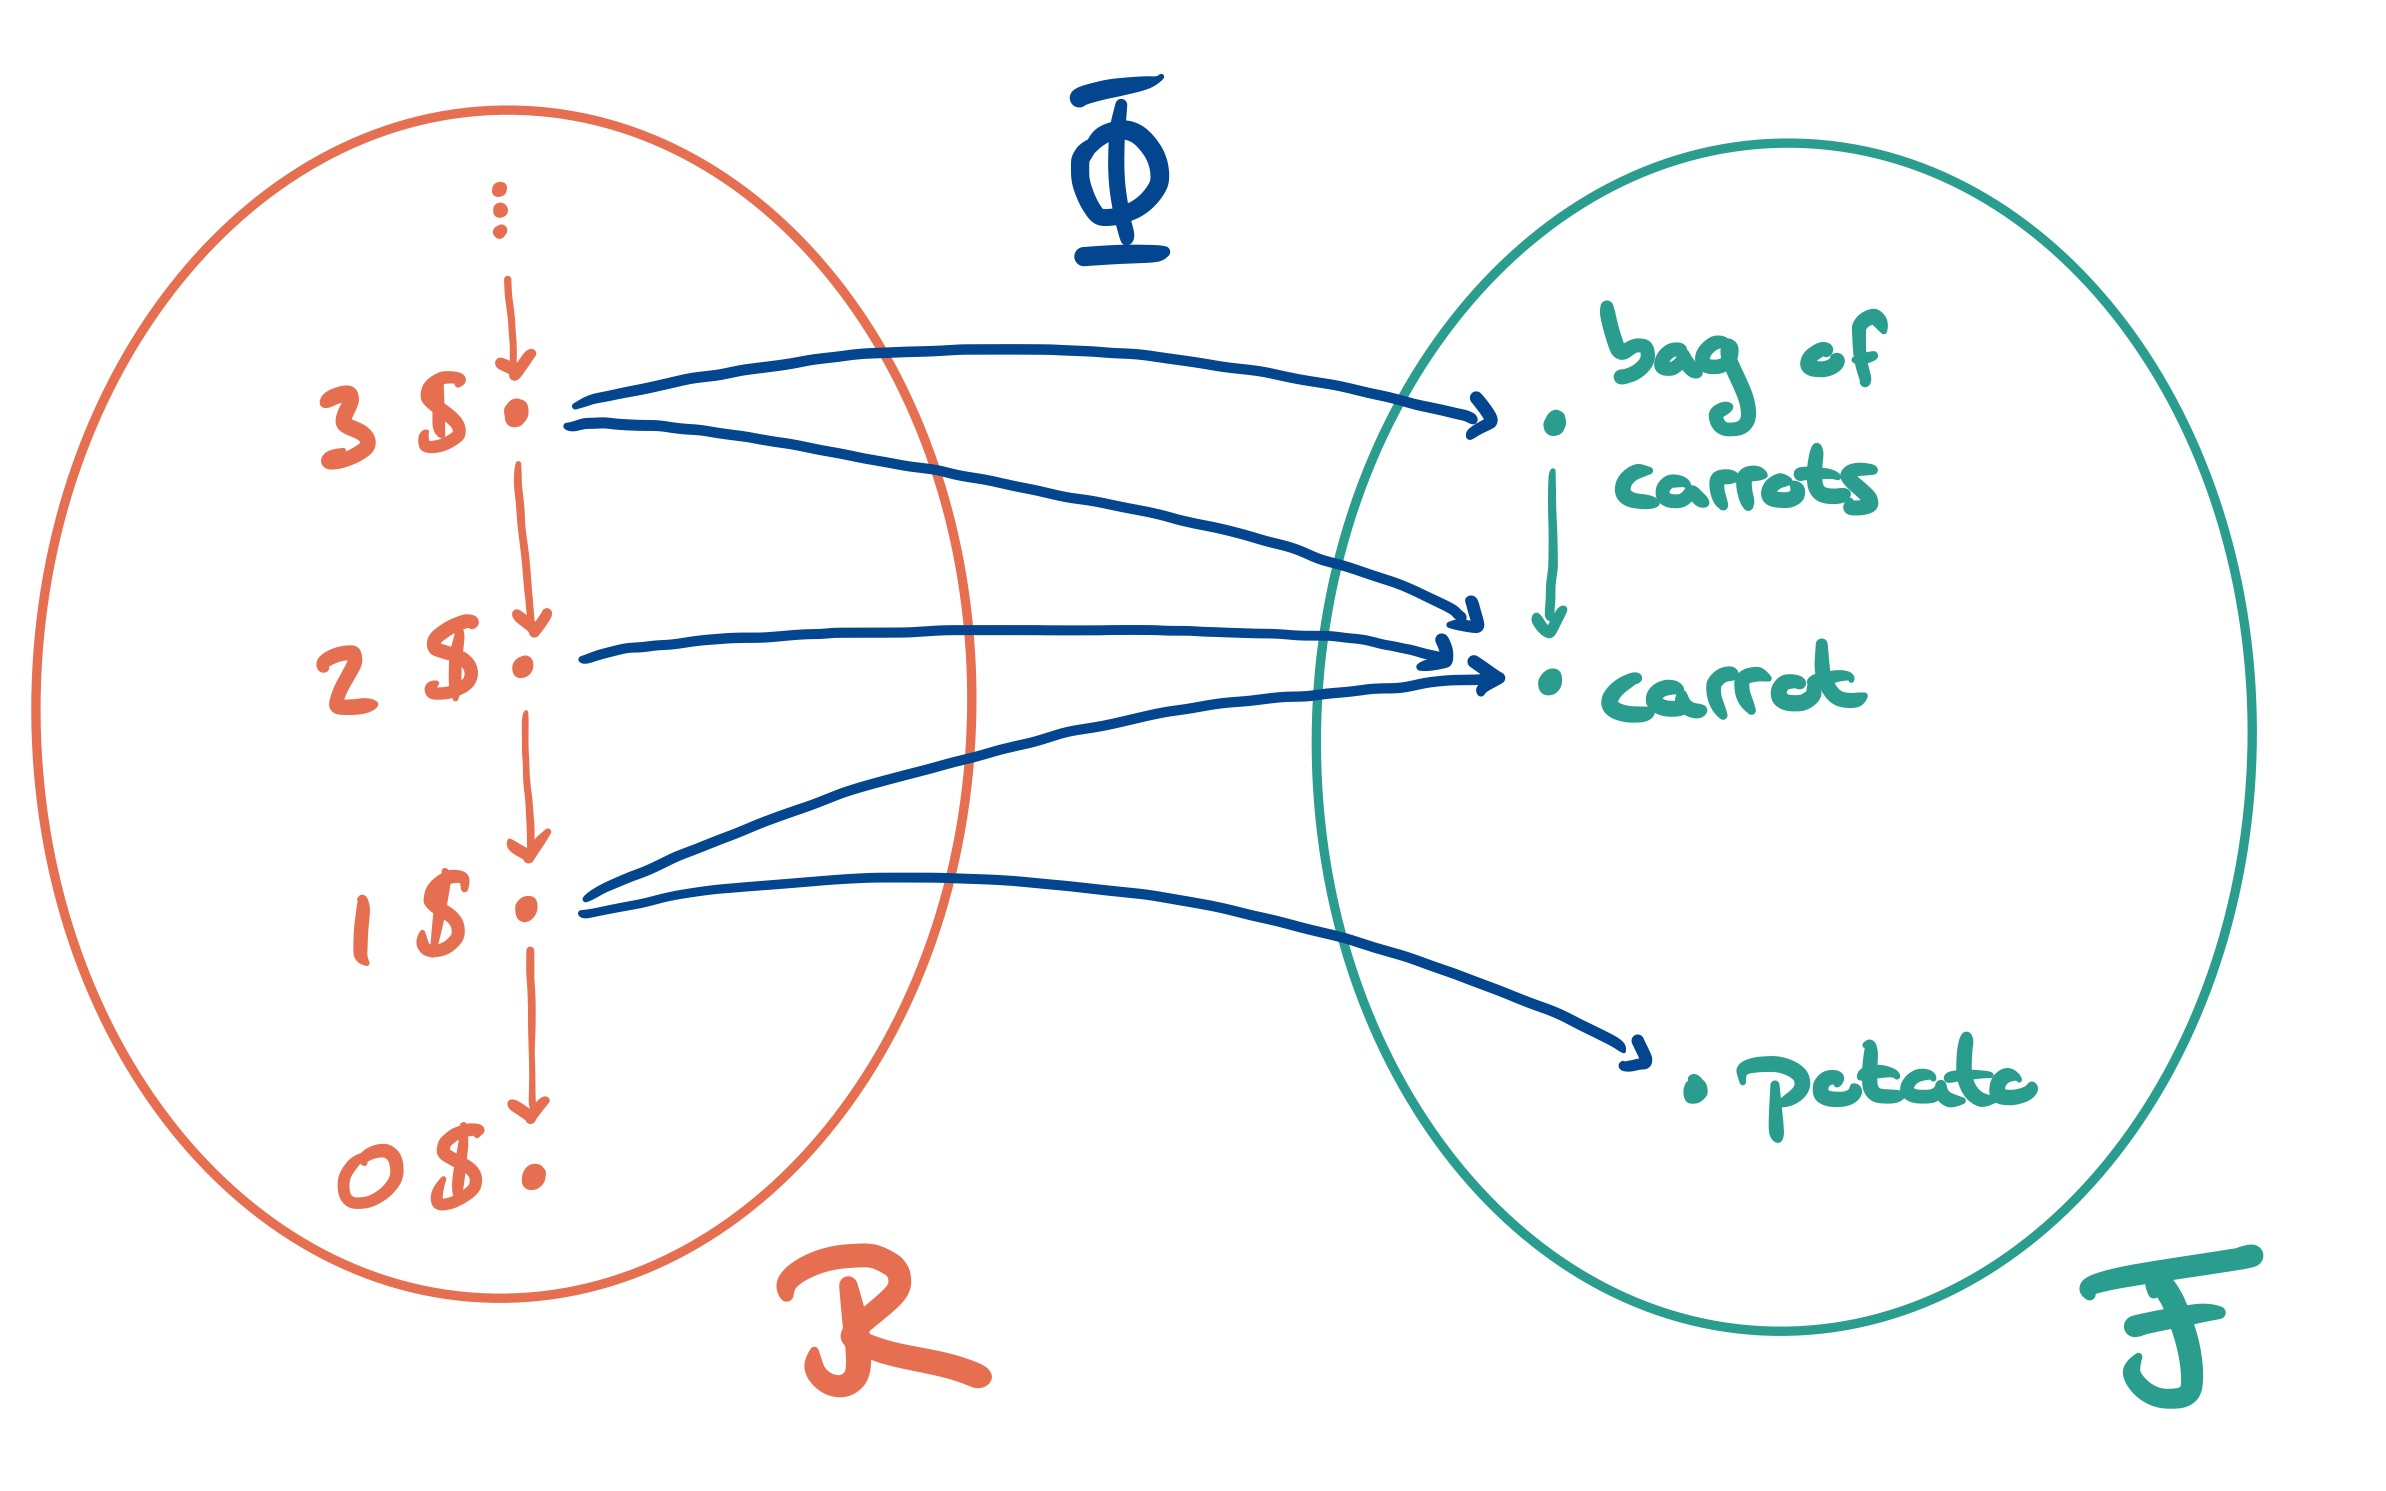
\includegraphics[width=350pt]{images/ex_groceries}
		\caption{Internal diagram of a feasibility relation $\Phi: \mc{R} \xslashedrightarrow{} \mc{F}$.}
		\label{fig:internal feas}
	\end{figure}

\end{continueexample}

We could have also defined feasibility relations as special types of monotone maps. For this we need to introduce several concepts.

\begin{definition}
	Let $\mathsf{Bool}$ denote the preorder generated by $\{\false \rightarrow \true\}$. Explicitly, $\mathsf{Bool}$ contains the arrows $\false \shortrightarrow \false$, $\false \shortrightarrow \true$, and $\true \rightarrow \true$.
\end{definition}

\begin{definition}[Opposite Preorder]
	Given a preorder $(\mc{P},\shortrightarrow)$, we define its \emph{opposite preorder} $\mc{P}^\text{op}$ to be the preorder that is obtained by reversing all the arrows in $\mc{P}$. That is, we set $a \shortrightarrow b$ in $\mc{P}^\text{op}$ if and only if $b \shortrightarrow a$ in $\mc{P}$. 
\end{definition}

\begin{definition}[Product of Preorders]
	Let $\mc{P}$ and $\mc{Q}$ be preorders. Their \emph{product} $\mc{P} \times \mc{Q}$ consists of all pairs $(p,q)$ where $p \in \mc{P}$ and $q \in \mc{Q}$ where we set $(p,q) \shortrightarrow (p',q')$ if and only if $p \shortrightarrow p'$ in $\mc{P}$ and $q \shortrightarrow q'$ in $\mc{Q}$.
\end{definition}

\begin{definition}[Monotone Map]
	Let $\mc{P}$ and $\mc{Q}$ be preorders. A function $f: \mc{P} \rightarrow \mc{Q}$ is called \emph{monotone} if it preserves the order in $\mc{P}$. That is, whenever $a \shortrightarrow b$ in $\mc{P}$, we have $f(a) \shortrightarrow f(b)$ in $\mc{Q}$.
\end{definition}

\begin{lemma}
	There is a one-to-one correspondence between feasibility relations $\Phi: \mc{R} \xslashedrightarrow{} \mc{F}$ and monotone maps $\mc{R}^\text{op} \times \mc{F} \rightarrow \mathsf{Bool}$.
\end{lemma}
\begin{proof}
	Given a feasibility relation $\Phi: \mc{R} \xslashedrightarrow{} \mc{F}$ as defined in Definition \ref{def:feasibility}, we obtain a function $F: \mc{R}^\text{op} \times \mc{F} \rightarrow \mathsf{Bool}$ by sending $(r,f) \mapsto \true$ if and only if $(r,f) \in \Phi$. Conditions (i) and (ii) of Definition \ref{def:feasibility} say that this function is monotone. Conversely, given a monotone map $F: \mc{R}^\text{op} \times \mc{F} \rightarrow \mathsf{Bool}$, we can obtain a relation $\Phi$ by setting $(r,f) \in \Phi$ if and only if $F(r,f) = \true$. The monotonicity of this function implies that $\Phi$ satisfies conditions (i) and (ii). It is apparent that these processes are inverse to one another.
\end{proof}

\begin{tcolorbox}[title=Feasibility Relations, colframe=Apricot, colback = paleorange, coltitle = Sepia]
	A feasibility relation $\Phi: \mc{R} \xslashedrightarrow{} \mc{F}$ expresses which functionalities in $\mc{F}$ can be obtained from which resources in $\mc{R}$. We write $\Phi(r,f) = \mathtt{true}$ to indicate that $f \in \mc{F}$ can be obtained from $r \in \mc{R}$. The relation $\Phi$ needs to satisfy the two monotonicity conditions in Definition \ref{def:feasibility} which can be concisely expressed by saying the $\Phi$ is a monotone map $\mc{R}^\text{op} \times \mc{F} \rightarrow \mathsf{Bool}$.
\end{tcolorbox}

\section{Choice between Resources}
We now extend what we've seen so far to encompass choice and uncertainty. What is meant by these terms is best illustrated with an example.

\begin{example}[Menu Options]\label{ex:menu}
	A restaurant might offer the following menu options:
	\begin{itemize}
		\item Coffee or tea (customer choice)
		\item Asparagus or pumpkin soup (depending on availability)
	\end{itemize}
	In the first case, we as customers are given the choice between coffee or tea. In the second, it is chosen for us which soup we will get, depending on what the cooks have available. From our perspective as customers, this represents an uncertainty. In both cases, however, we will end up with exactly one of the options. \exampleend
\end{example}

We might refer to the two modes of choice presented in Example \ref{ex:menu} as \emph{free choice} and \emph{forced choice}, respectively. Alternatively, we could call them \emph{choice} and \emph{uncertainty}, or \emph{internal} and \emph{external} choice. Regardless of the names we choose, the terms are relative to which perspective we are taking. If we look through the eyes of the restaurant, the customer choice of coffee or tea is external, while the choice of soup is internal.

\subsection{Choice Connectives}
Suppose we are given some preorder $\mc{P}$ of resources or functionalities. Our goal will be to augment $\mc{P}$ to include all possible free and forced choices among subsets $A \sub \mc{P}$. Let us call this choice-augmented preorder $\mathsf{C}(\mc{P})$. To this end we introduce two connectives to express free and forced choice.

\begin{definition}[Choice Connectives] Given a set $A$, we denote
	\begin{itemize}
		\item the \emph{free choice} among $a \in A$ by $\cbigsqcap{a \in A} a$,
		\item the \emph{forced choice} among $a \in A$ by $\cbigsqcup{a \in A} a$.
	\end{itemize}
	When $A=\{a_1,\ldots,a_n\}$ is finite, we will also write 
	$$a_1 \csqcap \ldots \csqcap a_n := \cbigsqcap{a \in A} a,$$
	$$a_1 \csqcup \ldots \csqcup a_n := \cbigsqcup{a \in A} a.$$
\end{definition}

We would like $\mathsf{C}(\mc{P})$ to contain all elements of $\mc{P}$ along with a single element for each possible choice. Moreover, we would like the preorder structure on $\mathsf{C}(\mc{P})$ to fit our established interpretation: An arrow $a \shortrightarrow b$ in $\mathsf{C}(\mc{P})$ should signify that being able to provide $a$ implies being able to provide $b$. This poses the following questions:
\begin{itemize}
	\item[(i)] When are two choices as represented by the connectives distinct?
	\item[(ii)] When must we add an arrow $a \shortrightarrow b$ if $a$ or $b$ represent choices?
\end{itemize}
We will answer these questions in what follows, beginning with (ii).

\subsubsection{Arrows between Choices}\label{sec:intr free}
In this section we describe when we should add arrows in the choice-augmented preorder $\mathsf{C}(\mc{P})$. We start by considering free choice.

Suppose that we are able to provide a free choice among some set $A \sub \mathsf{C}(\mc{P})$. This means that regardless of which $a \in A$ is picked freely, we must be able to provide that $a$. In other words, being able to provide a free choice among $A$ implies being able to provide any $a \in A$. Formally,


\begin{equation}\label{eq:meet 1}
	\cbigsqcap{a \in A} a \shortrightarrow a, \quad \forall a \in A.
\end{equation}

Let $A \sub \mathsf{C}(\mc{P})$ and suppose that there is a fixed $t \in \mathsf{C}(\mc{P})$ such that for every $a \in A$, being able to provide $t$ implies being able to provide $a$. Being able to provide a free choice among $A$ means that whatever $a \in A$ is picked freely, we can provide that $a$. By assumption, if we can provide $t$, we are able to provide any $a \in A$, and hence also the free choice among $A$. Formally,
\begin{equation}\label{eq:meet 2}
	\forall a \in A : t \shortrightarrow a  \quad \Rightarrow \quad t \shortrightarrow 	\cbigsqcap{a \in A} a.
\end{equation}

We now turn to forced choice. Being able to provide a forced choice among $B \sub \mathsf{C}(\mc{P})$ means being able to provide some $b \in B$, without having to specify which. Therefore, being able to provide some $b \in B$ implies being able to provide a forced choice among $B$. Formally,
\begin{equation}\label{eq:join 1}
b \shortrightarrow \cbigsqcup{b \in B} b, \quad \forall b \in B.
\end{equation}

Finally, suppose that for every $b \in B$, being able to provide $b$ implies being able to provide a fixed $t \in \mathsf{C}(\mc{P})$. Assume we can provide a forced choice among $B$. This means that we are able to provide some $b \in B$. However, regardless of which $b$ we are able to provide, our hypothesis says that this implies we are able to provide $t$. Therefore, being able to provide a forced choice among $B$ implies being able to provide $t$. Formally, 
\begin{equation}\label{eq:join 2}
\forall b \in B : b \shortrightarrow t  \quad \Rightarrow \quad  \cbigsqcup{b \in B} b \shortrightarrow t.
\end{equation}


We now observe that (\ref{eq:meet 1}) and (\ref{eq:meet 2}) mean that $\csqcap$ is the \emph{meet} over $a \in A$, while (\ref{eq:join 1}) and (\ref{eq:join 2}) show that $\csqcup$ is the \emph{join} over $b \in B$.

\begin{definition}[Meets and Joins]\label{def:meets joins}
	Let $(\mc{P},\shortrightarrow)$ be a preorder and $A \sub \mc{P}$. A \emph{meet} of the set $A$ is an element $\bigwedge_{a \in A} a$ in $\mc{P}$ such that
	\begin{itemize}
		\item[(i)] $\bigwedge_{a \in A} a$ is a lower bound of $A$, that is $\bigwedge_{a \in A} a  \shortrightarrow a$ for all $a \in A$,
		\item[(ii)] $\bigwedge_{a \in A} a$ is the greatest lower bound of $A$, that is if $t \shortrightarrow a$ for all $a \in A$, then $t \shortrightarrow \bigwedge_{a \in A} a$.
	\end{itemize}
	A \emph{join} of the set $A$ is an element $\bigvee_{a \in A} a$ in $\mc{P}$ such that
	\begin{itemize}
		\item[(i)] $\bigvee_{a \in A} a$ is an upper bound of $A$, that is $a  \shortrightarrow \bigvee_{a \in A} a$ for all $a \in A$,
		\item[(ii)] $\bigvee_{a \in A} a$ is the least upper bound of $A$, that is if $a \shortrightarrow t$ for all $a \in A$, then $\bigvee_{a \in A} a \shortrightarrow t$.
	\end{itemize}
	A preorder in which every subset has a meet and a join is called a \emph{complete lattice}.
\end{definition}

Our discussion shows that our choice-augmented preorder $\mathsf{C}(P)$ will have meets and joins for any subset $A \sub \mathsf{C}(\mc{P})$. Therefore, $\mathsf{C}(P)$ will be a complete lattice.

\subsubsection{Equality of Choices}\label{sec:intr self}
The fact that free and forced choices are meets and joins in $\mathsf{C}(\mc{P})$ already implies many equalities between expressions consisting of the connectives $\csqcap$ and $\csqcup$. In this section we will show that in addition to these we also want the connectives to distribute over one another.

Suppose we have a series of choices given by $a \csqcap (b \csqcup c)$. This means we get to freely choose between getting $a$ for certain, or between the uncertainty of getting $b$, or $c$. In this scenario, we can always guarantee $a$ if we want, but we are uncertain whether we will get $b$ or $c$, if we don't choose $a$. Compare this with the series of choices given by $(a \csqcap b) \csqcup (a \csqcap c)$. Here too we can always guarantee $a$, but are uncertain whether we will get $b$ or $c$, if we don't choose $a$. In fact, in terms of which resources we can guarantee, the two formulations are equivalent from our perspective. Hence, we can assume the following distributive law $$a \csqcap (b \csqcup c) = (a \csqcap b) \csqcup (a \csqcap c).$$

Dually, we can compare $a \csqcup (b \csqcap c)$ with $(a \csqcup b) \csqcap (a \csqcup c)$. In the first expression we are uncertain whether we will get $a$, or a free choice between $b$ and $c$. This means that if we don't get $a$, we can guarantee either $b$ or $c$. This is also the case in the second expression. Hence, we may assume the distributive law $$a \csqcup (b \csqcap c) = (a \csqcup b) \csqcap (a \csqcup c).$$

More generally, these laws should also hold for the infinite case. The statement of the infinite distributive law is more complicated: For any doubly indexed family of elements $\{b_{j,k} : j \in J, k \in K_j\}$ of $\mathsf{C}(\mc{P})$ we have
\begin{equation}\label{eq:meet dist}
	\cbigsqcap{j \in J} \left( \cbigsqcup{k \in K_j} b_{j,k} \right) = \cbigsqcup{f \in F} \left( \cbigsqcap{j \in J} b_{j,f(j)} \right),
\end{equation}
where $F$ is the set of all choice functions choosing for each index $j \in J$ some index $f(j) \in K_j$.

This law is justified by the following argument. Suppose we are presented with a choice of the form $\cbigsqcap{j \in J} \left( \cbigsqcup{k \in K_j} b_{j,k} \right)$. Then we can guarantee $\cbigsqcup{k \in K_j} b_{j,k} $ for any $j \in J$ we choose. That is we can guarantee an uncertainty between the $b_{j,k}$ for one specific $j$ of our choice. Now consider $\cbigsqcup{f \in F} \left( \cbigsqcap{j \in J} b_{j,f(j)} \right)$. Here, some $f \in F$ is chosen for us. We then get to chose freely between the $b_{j,f(j)}$ for that fixed $f$. Hence we still have uncertainty among a set of $b_{j,k}$ for a $j$ of our choice. Moreover, $f$ picks precisely one $k = f(j)$ among all $k \in K_j$, so the set of $b_{j,k}$ for which there is uncertainty remains the same in both cases.

We can also formulate the dual distributive law
\begin{equation}\label{eq:join dist}
\cbigsqcup{j \in J} \left( \cbigsqcap{k \in K_j} b_{j,k} \right) = \cbigsqcap{f \in F} \left( \cbigsqcup{j \in J} b_{j,f(j)} \right),
\end{equation}
which happens to be equivalent to (\ref{eq:meet dist}) provided both $\cbigsqcap{a \in A}$ and $\cbigsqcup{a \in A}$ exist for any subset $A \sub \mathsf{C}(\mc{P})$.

In summary, our discussion shows that in addition to being a complete lattice, $\mathsf{C}(\mc{P})$ should also satisfy the infinite distributive laws (\ref{eq:meet dist}) and (\ref{eq:join dist}). A complete lattice satisfying infinite distributivity is called a \emph{completely distributive lattice}.

\begin{tcolorbox}[title=Choice Connectives, colframe=Apricot, colback = paleorange, coltitle = Sepia]
	We denote the \emph{free choice} among $a \in A$ by $\cbigsqcap{a \in A} a$, and 
	the \emph{forced choice} among $a \in A$ by $\cbigsqcup{a \in A} a$. The connective $\csqcap{}$ acts like a meet, while $\csqcup{}$ acts like a join. Moreover, both connectives distribute over one another, even in the infinite case.
\end{tcolorbox}

\subsection{A Universal Model for Choice}
Given a preorder $\mc{P}$, we want to construct a choice-augmented preorder $\mathsf{C}(\mc{P})$ that includes all possible choices between elements of $\mc{P}$. Our discussion in the previous section showed that $\mathsf{C}(\mc{P})$ should be a completely distributive lattice, where a free choice among a set $A$ is given by the meet over $A$, and a forced choice over a set $B$ is given by the join over $B$. Moreover, we want the new elements in $\mathsf{C}(\mc{P})$ to only fulfill those relations implied by our interpretation of these elements as choices. This leads us to consider the free completely distributive lattice generated by $\mc{P}$.

There are several notions of free completely distributive lattice one could use, depending on what set of maps one is interested in. We will follow \cite{Morris2004}, which shows that the upper sets of lower sets of $\mc{P}$, denoted $\upper(\low(\mc{P}))$, satisfy a universal property that suits our purposes. We will explain this in more detail after making the requisite definitions.

We start by defining special subsets of a preorder which are upwards and downward closed.
\begin{definition}[Upper and Lower Sets]
	Let $\mc{P}$ be a preorder. A subset $U \sub \mc{P}$ is called an \emph{upper set}, if it is upward closed: 
	$$x \in U \text{ and } x \shortrightarrow y  \text{ imply } y \in U.$$
	A subset $L \sub \mc{P}$ is called a lower set, if it is downward closed:
	$$x \in L \text{ and } y \shortrightarrow x  \text{ imply } y \in L.$$
\end{definition}

\begin{definition}[Upper and Lower Closure]
	Given a subset $A \sub \mc{P}$ of a preorder, we can form its
	\begin{itemize}
		\item \emph{upper closure} $\upc{A} := \{p \in \mc{P} : a \shortrightarrow p \text{ for some } a \in A\}$,
		\item \emph{lower closure} $\lwc{A} := \{p \in \mc{P} : p \shortrightarrow a \text{ for some } a \in A\}$.
	\end{itemize}
	The upper closure is an upper set, while the lower closure is a lower set. Moreover, we can consider
	\begin{itemize}
		\item upper sets $\upper\mc{P} := \{U \sub \mc{P}: U \text{ an upper set}\}$,
		\item lower sets $\low\mc{P} := \{L \sub \mc{P}: L \text{ an lower set}\}$.
	\end{itemize}
\end{definition}

We will be interested in monotone maps $f: \mc{P} \rightarrow \mc{Q}$ in which the implication ``$p \shortrightarrow q$ implies $f(p) \shortrightarrow f(q)$'' is actually an equivalence.
\begin{definition}[Order Embedding]
	Let $\mc{P}$ and $\mc{Q}$ be preorders. A function $f: \mc{P} \rightarrow \mc{Q}$ is called an order embedding provided
	$$ p \shortrightarrow q \Leftrightarrow f(p) \shortrightarrow f(q) .$$
	In this case we write $f: \mc{P} \hookrightarrow \mc{Q}$.
\end{definition}

\begin{lemma}\label{lem:upper lower lattice}
	Given a preorder $\mc{P}$, its upper sets can be preordered by containment $(\upper\mc{P}, \supseteq)$ and its lower sets can be ordered by inclusion $(\low\mc{P}, \sub)$. Both of these structures are completely distributive lattices. Moreover, we have order embeddings: 
	$$i_\mathsf{U}: \mc{P} \hookrightarrow (\upper\mc{P}, \supseteq) \qquad \qquad i_\mathsf{L}: \mc{P} \hookrightarrow (\low\mc{P}, \sub)$$
	$$ p \mapsto \upc{\{p\}} \qquad \qquad \qquad p \mapsto \lwc{\{p\}}$$
\end{lemma}
\begin{proof}
	We will take for granted that the power set $(\mathsf{P}(\mc{P}),\sub)$, ordered by inclusion, is a completely distributive lattice with set intersection as meet and set union as join. This follows from a straightforward check of the definition for meets and joins (Def.~\ref{def:meets joins}) and verification of the infinite distributive laws (\ref{eq:meet dist}) and (\ref{eq:join dist}). We now observe that unions and intersections of upper sets are again upper sets. The same holds for lower sets. Therefore, the completely distributive structure on $(\mathsf{P}(\mc{P}),\sub)$ restricts to completely distributive lattices $(\upper\mc{P}, \sub)$ and $(\low\mc{P}, \sub)$. Finally, since $(\upper\mc{P}, \sub)^\text{op} = (\upper\mc{P}, \supseteq)$ and the defining laws for completely distributive lattices are self-dual, we see that also $(\upper\mc{P}, \supseteq)$ is completely distributive.
	
	To prove that $i_\mathsf{U}$ is an order embedding let $p \shortrightarrow q$ in $\mc{P}$. Suppose $x \in \upc{\{q\}}$. Then $q \shortrightarrow x$, whence $p \shortrightarrow x$ by transitivity. Hence, $x \in \upc{\{p\}}$, so $\upc{\{p\}} \supseteq \upc{\{q\}}$. Conversely, if $\upc{\{p\}} \supseteq \upc{\{q\}}$, then in particular $q \in \upc{\{p\}}$, since $q \in \upc{\{q\}}$. Hence $p \shortrightarrow q$, as desired. The proof that $i_\mathsf{L}$ is an order embedding is analogous.
\end{proof}

We now have the tools to understand the free completely distributive lattice constructed in \cite{Morris2004}. Lemma \ref{lem:upper lower lattice} shows that given a preorder $\mc{P}$, we can obtain a completely distributive lattice $(\low\mc{P}, \sub)$. Since this is again a preorder, we can reapply the lemma and consider the completely distributive lattice $(\upper\low\mc{P}, \supseteq)$. In fact, \cite{Morris2004} shows that $\upper\low\mc{P}$ satisfies the following universal property:
\begin{quote}
	There is an order embedding $i: \mc{P} \hookrightarrow \upper\low\mc{P}$, such that for any monotone function $f: \mc{P} \rightarrow M$ into a completely distributive lattice $M$, there is a unique complete homomorphisms $u: \upper\low\mc{P} \rightarrow M$ (preserving arbitrary meets and joins) satisfying $u \circ i = f$.
\end{quote}

If we augment a preorder $\mc{P}$ to include choice, we should have a monotone map $c: \mc{P} \rightarrow \mathsf{C}(\mc{P})$ which maps each element of $\mc{P}$ to the free (or forced) choice among the singleton $\{p\}$. Therefore, by the universal property above, there will be a unique map from $u: \upper\low\mc{P} \rightarrow \mathsf{C}(\mc{P})$, preserving the elements of $\mc{P}$ and the choices among them. 

To see what this means, consider a free choice over $A \sub \mc{P}$. This will be represented by the meet $\bigwedge_{a \in A} c(a)$ in $\mathsf{C}(\mc{P})$, and by $\bigwedge_{a \in A} i(a)$ in $\upper\low\mc{P}$. Since the unique map $u$ preserves meets, and $u \circ i = c$, we have
$$u \left ( \bigwedge_{a \in A} i(a) \right) = \bigwedge_{a \in A} u(i(a)) = \bigwedge_{a \in A} c(a).$$
Hence each free choice represented in $\mathsf{C}(\mc{P})$ is the image of the corresponding choice represented in $\upper\low\mc{P}$. The same holds for forced choices. This shows that the part of $\mathsf{C}(\mc{P})$ we are interested lies in is the image of $\upper\low\mc{P}$ under the unique map $u$. In this sense, $\upper\low\mc{P}$ serves as a universal model for choice on $\mc{P}$, which we will call the \emph{upper-lower model}.

\begin{tcolorbox}[title=Universal Model for Choice, colframe=Apricot, colback = paleorange, coltitle = Sepia]
	Given a preorder $\mc{P}$ we can form the \emph{upper-lower model} $\upper\low\mc{P}$, given by the upper sets (ordered by containment) of the lower sets (ordered by inclusion) of $\mc{P}$. For any other model $\mathsf{C}(\mc{P})$ of choice on $\mc{P}$, the free and forced choices in $\mathsf{C}(\mc{P})$ lie in the image of $\upper\low\mc{P}$ under a unique map. 
\end{tcolorbox}

\subsection{The Upper-Lower Model}\label{sec:upper-lower model}
Apart from being universal, the upper-lower model lends itself to easy interpretation. This section will describe how. In addition, we present rules which simplify the evaluation of choices. \\

Given a preorer $\mc{P}$, we consider the upper-lower model $\upper\low\mc{P}$. By Lemma \ref{lem:upper lower lattice} we have an order embedding $i: \mc{P} \hookrightarrow \upper\low\mc{P}$ given by $p \mapsto \upc{\lwc{\{p\}}}$. In addition, we know that meets and joins in $\upper\low\mc{P}$ are given by unions and intersections, respectively. Hence, we implement our connectives $\csqcap$ and $\csqcup$ by setting 
$$ \cbigsqcap{a \in A} a :=  \bigcup_{a \in A} a,$$
$$ \cbigsqcup{a \in A} a := \bigcap_{a \in A} a.$$

In particular, if we are interested choice between elements of $\mc{P}$, we first embed those elements into $\upper\low\mc{P}$ and then apply the corresponding operation. That is if $B \sub \mc{P}$,
$$ \cbigsqcap{p \in B} p :=  \bigcup_{p \in B} i(p),$$
$$ \cbigsqcup{p \in B} p := \bigcap_{p \in B} i(p).$$
\begin{remark}
	Observe that we are overloading the symbols $\csqcap$ and $\csqcup$ to express both choice between elements of $\upper\low\mc{P}$ and $\mc{P}$. The two uses only differ by the embedding $i: \mc{P} \hookrightarrow \upper\low\mc{P}$. It should be clear from context which meaning applies. 
\end{remark}

If $\mc{P}$ is finite, an element of $\upper\low\mc{P}$ has the form
$$\color{OliveGreen} \bm{\{} \color{Black} \color{BrickRed} \bm{\{} \color{Black} p_{1,1}, \ldots, p_{1,n_1} \color{BrickRed} \bm{\}} \color{Black}, \ldots, \color{BrickRed} \bm{\{} \color{Black} p_{m,1}, \ldots, p_{m,n_m} \color{BrickRed} \bm{\}} \color{Black}  \color{OliveGreen} \bm{\}} \color{Black}$$
where the green brackets indicate an upper set, while the red brackets indicate lower sets. In the general case, an element of $\upper\low\mc{P}$ has the form
\begin{equation}\label{eq:ulp element}
	\color{OliveGreen} \bm{\{} \color{Black} \color{BrickRed} \bm{\{} \color{Black} p_{k,j} \color{BrickRed} \bm{\}}_{k \in K_j} \color{Black}  \color{OliveGreen} \bm{\}}_{j \in J} \color{Black}
\end{equation}
where again green indicates an upper set and red indicates lower sets.

We will interpret an the element (\ref{eq:ulp element}) as the choice
$$\cbigsqcap{j \in J} \left( \: \cbigsqcup{k \in K_j} p_{j,k} \right).$$

To justify this interpretation, we will need the following

\begin{lemma}\label{lem:exchange upc}
	Let $(\mc{P},\shortrightarrow)$ be a preorder. Then for a collection $\{p_i\} \sub \mc{P}$,
	$$ \upc{\{p_i\}_{i \in I}} = \bigcup_{i \in I} \upc{\{p_i\}},$$
	$$ \lwc{\{p_i\}_{i \in I}} = \bigcup_{i \in I} \lwc{\{p_i\}}.$$
\end{lemma}
\begin{proof}
	Suppose $x \in \upc{\{p_i\}_{i \in I}}$. Then $p_i \shortrightarrow x$ for some $i \in I$, whence $x \in \upc{\{p_i\}} \sub \bigcup_{i \in I} \upc{\{p_i\}}$. Conversely, if $x \in \bigcup_{i \in I} \upc{\{p_i\}}$, then $x \in \upc{\{p_i\}}$ for some $i \in I$. This means $p_i \shortrightarrow x$, whence $x \in \upc{\{p_i\}_{i \in I}}$. The second statement follows by applying the first to $\mc{P}^\text{op}$.
\end{proof}

\begin{lemma}\label{lem:intersection as union}
	Let $\mc{P}$ be a preorder.
	\begin{itemize}
		\item[(i)] If $\{ A_i \}_{i \in I} \sub \upper\low\mc{P}$ is a collection of elements of the upper-lower model, then
		$$\bigcap_{i \in I} A_i = \{ \bigcup_{i \in I} a_i : a_i \in A_i \text{ for each } i \in I \} .$$
		\item[(ii)] If $\{a_j\}_{j \in J} \sub \low\mc{P}$ is a collection of lower sets, then
		$$\bigcap_{j \in J} \upc{\{a_j\}} =\upc{ \{ \bigcup_{j \in J} a_j \}} .$$
		\item[(iii)] If $\{p_k\}_{k \in K} \sub \mc{P}$ is a collection of elements of $\mc{P}$, then
		$$\bigcap_{k \in K} \upc{\{ \lwc{\{p_k\}} \}} =\upc{ \{ \lwc{ \{p_k\}_{k \in K} } \}} .$$
	\end{itemize}	
\end{lemma} 
\begin{proof}
	To show (i), suppose $x \in \bigcap_{i \in I} A_i$. Then $x \in A_i$ for each $i \in I$. Writing $x = \bigcup_{i \in I} x$ shows that $x \in \{ \bigcup_{i \in I} a_i : a_i \in A_i \text{ for each } i \in I \}$. Conversely, consider $x = \bigcup_{i \in I} a_i$ where $a_i \in A_i$ for all $i \in I$. Recall that the $A_i$ are upper sets of $(\low\mc{P},\sub)$. Hence $a_i \in A_i$ and $a_i \sub \bigcup_{i \in I} a_i = x$ imply $x \in A_i$. This holds for every $i \in I$, so $x \in \bigcap_{i \in I} A_i$.
	
	For (ii), we note that by (i), 
	$$\bigcap_{i \in I} \upc{\{a_j\}} = \{ \bigcup_{j \in J} b_j : b_j \in \upc{\{a_j\}}  \text{ for each } j \in J \}.$$
	Since $b_j \in \upc{\{a_j\}}$ means $b_j \supseteq a_j$, we have
	$$\bigcap_{i \in I} \upc{\{a_j\}} = \{ \bigcup_{j \in J} b_j : b_j \supseteq a_j \text{ for each } j \in J \}.$$ 
	Suppose $x = \bigcup_{j \in J} b_j$, where $b_j \supseteq a_j$ for all $j \in J$. Then $\bigcup_{j \in J} b_j \supseteq \bigcup_{j \in J} a_j $, whence $x \in \upc{ \{ \bigcup_{j \in J} a_j \}}$. Conversely, if $x \supseteq \bigcup_{j \in J} a_j$, then $x \supseteq  a_j$ for each $j \in J$. Therefore, $x = \bigcup_{j \in J} x$ is an element of $\{ \bigcup_{j \in J} b_j : b_j \supseteq a_j \text{ for each } j \in J \}$. In summary,
	$$\bigcap_{i \in I} \upc{\{a_j\}} = \{ \bigcup_{j \in J} b_j : b_j \supseteq a_j \text{ for each } j \in J \} = \upc{ \{ \bigcup_{j \in J} a_j \}}.$$ 
	
	For (iii), we apply (ii) and Lemma \ref{lem:exchange upc} to obtain
	$$ \bigcap_{k \in K} \upc{\{ \lwc{\{p_k\}} \}} =  \upc{ \{ \bigcup_{k \in K} \lwc{\{p_k\}} \}} = \upc{ \{ \lwc{ \{p_k\}_{k \in K} } \}}.$$
\end{proof}


Returning to the interpretation, consider the element
$$ \color{OliveGreen} \bm{\{} \color{Black} \color{BrickRed} \bm{\{} \color{Black} p_{j,k} \color{BrickRed} \bm{\}}_{k \in K_j} \color{Black}  \color{OliveGreen} \bm{\}}_{j \in J} \color{Black}.$$
Since the red brackets are a lower set and the green brackets an upper set, we can rewrite
$$ \color{OliveGreen} \bm{\{} \color{Black} \color{BrickRed} \bm{\{} \color{Black} p_{j,k} \color{BrickRed} \bm{\}}_{k \in K_j} \color{Black}  \color{OliveGreen} \bm{\}}_{j \in J} \color{Black} = \upc{ \color{OliveGreen} \bm{\{} \color{Black} \lwc{\color{BrickRed} \bm{\{} \color{Black} p_{j,k} \color{BrickRed} \bm{\}}_{k \in K_j} \color{Black}}  \color{OliveGreen} \bm{\}}_{j \in J} \color{Black}}.$$
Using Lemmas \ref{lem:exchange upc} and  \ref{lem:intersection as union} (ii),
\begin{IEEEeqnarray*}{rCl}
	 \color{OliveGreen} \bm{\{} \color{Black} \color{BrickRed} \bm{\{} \color{Black} p_{j,k} \color{BrickRed} \bm{\}}_{k \in K_j} \color{Black}  \color{OliveGreen} \bm{\}}_{j \in J} \color{Black} & = & \upc{ \color{OliveGreen} \bm{\{} \color{Black} \lwc{\color{BrickRed} \bm{\{} \color{Black} p_{j,k} \color{BrickRed} \bm{\}}_{k \in K_j} \color{Black}}  \color{OliveGreen} \bm{\}}_{j \in J} \color{Black}} \\
	 & = & \bigcup_{j \in J} \upc{ \color{OliveGreen} \bm{\{} \color{Black} \bigcup_{k \in K_j} \lwc{\color{BrickRed} \bm{\{} \color{Black} p_{j,k} \color{BrickRed} \bm{\}} \color{Black}}  \color{OliveGreen} \bm{\}} \color{Black}} \\
	 & = & \bigcup_{j \in J} \bigcap_{k \in K_j} \upc{ \color{OliveGreen} \bm{\{} \color{Black} \lwc{\color{BrickRed} \bm{\{} \color{Black} p_{j,k} \color{BrickRed} \bm{\}} \color{Black}}  \color{OliveGreen} \bm{\}} \color{Black}} \\
	 & = & \cbigsqcap{j \in J} \left( \: \cbigsqcup{k \in K_j} p_{j,k} \right).
\end{IEEEeqnarray*}
This equation confirms our interpretation. \\


We now know how to interpret elements of $\upper\low\mc{P}$. We will now show how free and forced are represented in the upper lower model. Suppose $\{p_j\}_{j \in J}$ is a collection of elements in $\mc{P}$. Each $p_j$ embeds into $\upper\low\mc{P}$ as $\upc{\{\lwc{\{p_j\}}\}}$. The free choice among $\{p_j\}_{j \in J}$ is represented by 
\begin{equation}\label{eq:repr free}
	\cbigsqcap{j \in J} p_j = \bigcup_{j \in J} \upc{\{\lwc{\{p_j\}}\}} = \upc{\{\lwc{\{p_j\}}\}_{j \in J}},
\end{equation}
where we applied Lemma \ref{lem:exchange upc}.

On the other hand, the forced choice among these is given by
\begin{equation}\label{eq:repr forced}
	\cbigsqcup{j \in J} p_j = \bigcap_{j \in J} \upc{\{\lwc{\{p_j\}}\}} =\upc{\{ \lwc{\{ p_j \}_{j \in J} } \}}, 
\end{equation}
where we have used Lemma \ref{lem:intersection as union} (iii). \\

Let us see how this works in practice.
\begin{example}[Menu 2]
	In a restaurant we are allowed to choose between a vegetarian and a meat option. If we choose the vegetarian option, the restaurant will provide us a curry dish, or a casserole, depending on availability. If we choose the meat option we will get chicken or beef, depending on availability. Using our connectives, we can describe this as
	$$ (\mathtt{curry} \csqcup \mathtt{casserole}) \csqcap (\mathtt{chicken} \csqcup \mathtt{beef}).$$
	We model our options as the discrete preorder 
	$$\mc{P} := \{\mathtt{curry}, \mathtt{casserole}, \mathtt{chicken}, \mathtt{beef}\}.$$ 
	 Using rule (\ref{eq:repr forced}) describe above, we represent this choice in $\upper\low\mc{P}$ by
	 \begin{IEEEeqnarray*}{rCl}
	 	\mathtt{curry} \csqcup \mathtt{casserole} & = & \uparrow \{\lwc{\{\mathtt{curry},\mathtt{casserole}\}}\}\\
	 	& =& \uparrow \{\{\mathtt{curry},\mathtt{casserole}\}\}.
	 \end{IEEEeqnarray*}
 	A similar calculation shows $\mathtt{chicken} \csqcup \mathtt{beef} = \uparrow\{\{\mathtt{chicken},\mathtt{beef}\}\}$. Hence,
 	\begin{IEEEeqnarray*}{rCl}
 		(\mathtt{curry} \csqcup \mathtt{casserole}) &\csqcap& (\mathtt{chicken} \csqcup \mathtt{beef}) \\ &=& \upc{ \{\{\mathtt{curry},\mathtt{casserole}\}\}} \cup \upc{\{\{\mathtt{chicken},\mathtt{beef}\}\}} \\
 		&=& \uparrow\{\{\mathtt{curry},\mathtt{casserole}\} , \{\mathtt{chicken},\mathtt{beef}\} \}. \exampleend
 	\end{IEEEeqnarray*}
\end{example}

\begin{example}[Menu 3]
	A restaurant offers two menus, depending on the day. As customers, we can freely choose any option on the current menu. Suppose the menu items the first menu are $\{\mathtt{curry}, \mathtt{beef}\}$ and those on the second are $\{\mathtt{casserole}, \mathtt{chicken}\}$. In terms of our connectives, this choice becomes
	$$ (\mathtt{curry} \csqcap \mathtt{beef}) \csqcup (\mathtt{casserole} \csqcap \mathtt{chicken}).$$
	Using rule (\ref{eq:repr free}) we represent
	\begin{IEEEeqnarray*}{rCl}
		\mathtt{curry} \csqcap \mathtt{beef} &=& \uparrow \{\lwc{\{\mathtt{curry}\}}, \lwc{\{\mathtt{beef}\}}\} \\
		&=& \uparrow \{\{\mathtt{curry}\}, \{\mathtt{beef}\}\}.
	\end{IEEEeqnarray*}
	Similarly, $\mathtt{casserole} \csqcap \mathtt{chicken} = \uparrow \{\{\mathtt{casserole}\}, \{\mathtt{chicken}\}\}$.
	Hence, using Lemma \ref{lem:intersection as union} (ii), 
	\begin{IEEEeqnarray*}{rCl}
		(\mathtt{curry} \csqcap \mathtt{beef}) &\csqcup& (\mathtt{casserole} \csqcap \mathtt{chicken}) \\
		&=& \upc{\{\{\mathtt{curry}\}, \{\mathtt{beef}\}\}} \cap \upc {\{\{\mathtt{casserole}\}, \{\mathtt{chicken}\}\}} \\
		&= &\uparrow \{ \{\mathtt{curry}, \mathtt{casserole}\}, \{\mathtt{curry,chicken}\}, \\&& \quad \{\mathtt{beef,casserole}\}, \{\mathtt{beef,chicken}\} \}. \exampleend
	\end{IEEEeqnarray*} 
\end{example}

As seen in the examples, it is easiest to represent upper and lower sets by upper and lower closures. The following calculation rules describe how to take choices among elements represented in this fashion.

\begin{tcolorbox}[title = \hypertarget{box:calc rules} {Calculation Rules} for Upper and Lower Closures, colframe=TealBlue, coltitle=Sepia, colback=paleteal] 
		Let $\mc{P}$ be a preorder and $\{A_j\}_{j \in J}$ and $\{A_k\}_{k \in K}$ be indexed families of subsets of $\mc{P}$. Then the following rules hold for finite choices in $\upper\low\mc{P}$:
		\begin{itemize}
			\item[(i)] $\upc{\{ \lwc{A_j} \}_{j \in J}} \csqcap \upc{\{ \lwc{A_k} \}_{k \in K}} = \upc \{ \lwc{A_i} \}_{i \in J \cup K}$
			\item[(ii)] $\upc{\{ \lwc{A_j} \}_{j \in J}} \csqcup \upc{\{ \lwc{A_k} \}_{k \in K}} = \upc \{ \lwc{(A_j \cup A_k)} \}_{j,k \in J \times K}$
		\end{itemize}
		More generally, if $\{ A_{j,k} \}_{j \in J, k \in K_j}$ is a double indexed family of subsets of $\mc{P}$, then the following rules apply for infinite choice in $\upper\low\mc{P}$:
		\begin{itemize}
			\item[(iii)] $\cbigsqcap{j \in J} \upc{\{ \lwc{A_{j,k}} \}_{k \in K_j}} = \upc \{ \lwc{A_i} \}_{i \in \bigcup K_j }$
			\item[(iv)] $\cbigsqcup{j \in J} \upc{\{ \lwc{A_{j,k}} \}_{k \in K_j}} = \upc \{ \lwc{ \bigcup_{j \in J} A_{j,f(j)}} \}_{f \in F}$ \newline where $F$ denotes the set of choice functions $f: J \rightarrow \coprod_{j \in J} K_j$ with $f(j) \in K_j$ for all $j \in J$.
\end{itemize}
\end{tcolorbox}
\begin{proof}
%	For (i) we observe that by Lemma \ref{lem:exchange upc},
%	\begin{IEEEeqnarray*}{rCl}
%		\upc{\{ \lwc{A_j} \}_{j \in J}} \csqcap \upc{\{ \lwc{A_k} \}_{k \in K}} &=& \upc{\{ \lwc{A_j} \}_{j \in J}} \cup \upc{\{ \lwc{A_k} \}_{k \in K}} \\
%		& = & \upc( \{\lwc{A_j}\}_{j \in J} \cup \{ \lwc{A_k} \}_{k \in K})  \\
%		& = & \upc \{ \lwc{A_i} \}_{i \in J \cup K}.
%	\end{IEEEeqnarray*}
%	
%	For (ii) we apply Lemmas \ref{lem:intersection as union} and \ref{lem:exchange upc},
%	\begin{IEEEeqnarray*}{rCl}
%		\upc{\{ \lwc{A_j} \}_{j \in J}} \csqcup \upc{\{ \lwc{B_k} \}_{k \in K}} &=& \upc{\{ \lwc{A_j} \}_{j \in J}} \cap \upc{\{ \lwc{B_k} \}_{k \in K}} \\
%		& = &	\upc{ \{ \lwc{A_j} \cup \lwc{B_k} \}_{j,k \in J \times K} } \\
%		& = &	\upc \{ \lwc{(A_j \cup B_k)} \}_{j,k \in J \times K}
%	\end{IEEEeqnarray*}
	Note that (i) and (ii) are special cases of (iii) and (iv). Regarding (ii), this follows because choice functions $\{j,k\} \rightarrow J \cup K$ correspond to elements of the cartesian product $J \times K$.
	
	For (iii) we observe that by Lemma \ref{lem:exchange upc},
	\begin{IEEEeqnarray*}{rCl}
		\cbigsqcap{j \in J} \upc{\{ \lwc{A_{j,k}} \}_{k \in K_j}} &=& \bigcup_{j \in J} \upc{\{ \lwc{A_{j,k}} \}_{k \in K_j}} \\
		& = & \upc{ \bigcup_{j \in J} \{ \lwc{A_{j,k}} \}_{k \in K_j}} \\
		& = & \upc \{ \lwc{A_i} \}_{i \in \bigcup K_j }
	\end{IEEEeqnarray*}

	For (iv) we apply Lemma \ref{lem:exchange upc}, the infinite distributive law (\ref{eq:join dist}), and Lemma \ref{lem:intersection as union},
	\begin{IEEEeqnarray*}{rCl}
		\cbigsqcup{j \in J} \upc{\{ \lwc{A_{j,k}} \}_{k \in K_j}} &=& \bigcap_{j \in J} \upc{\{ \lwc{A_{j,k}} \}_{k \in K_j}} \\
		& = & \bigcap_{j \in J} \bigcup_{k \in K_j} \upc \{ \lwc A_{j,k} \} \\
		& = & \bigcup_{f \in F} \bigcap_{j \in J} \upc \{ \lwc A_{j,f(j)}\} \\
		& = & \bigcup_{f \in F} \upc \{ \bigcup_{j \in J} \lwc{A_{j,f(j)}} \} \\
		& = & \upc  \{ \bigcup_{j \in J} \lwc{A_{j,f(j)}} \}_{f \in F} \\
		& = & \upc \{ \lwc{ \bigcup_{j \in J} A_{j,f(j)}} \}_{f \in F}
	\end{IEEEeqnarray*}	
\end{proof}

\begin{tcolorbox}[title=Working in the Upper-lower Model, colframe=Apricot, colback = paleorange, coltitle = Sepia]
Given a preorder $\mc{P}$ we we have an order embedding $i: \mc{P} \hookrightarrow \upper\low\mc{P}$ into its upper-lower model. Free and forced choices are implemented in $\upper\low\mc{P}$ as
$$ \cbigsqcap{a \in A} a :=  \bigcup_{a \in A} a,$$
$$ \cbigsqcup{a \in A} a := \bigcap_{a \in A} a.$$
A general element of $\upper\low\mc{P}$ has the form 
$
\color{OliveGreen} \bm{\{} \color{Black} \color{BrickRed} \bm{\{} \color{Black} p_{k,j} \color{BrickRed} \bm{\}}_{k \in K_j} \color{Black}  \color{OliveGreen} \bm{\}}_{j \in J} \color{Black}
$
and is interpreted as
$\cbigsqcap{j \in J} \: \cbigsqcup{k \in K_j} p_{j,k}.$ Choices in $\upper\low\mc{P}$ can be calculated using the rules presented in Lemmas \ref{lem:exchange upc}, \ref{lem:intersection as union}, and the \hyperlink{box:calc rules}{box above}.
\end{tcolorbox}

\section{Feasibility between Choices}
Given a preorders of resources $\mc{R}$ and functionalities $\mc{F}$, we are able to model free and forced choices by considering their upper-lower models $\upper\low\mc{R}$ and $\upper\low\mc{F}$. In this section, we will lift feasibility relations $\Phi: \mc{R} \xslashedrightarrow{} \mc{F}$ to the upper-lower models. We will obtain a new feasibility relation $\upper\low\Phi: \upper\low\mc{R} \xslashedrightarrow{} \upper\low\mc{F}$, which extends $\Phi$ to choice. Moreover, we will see that such lifted feasibility relations $\upper\low\Phi$ enjoy special properties that distinguish them from arbitrary feasibility relations between the upper-lower models. Finally, we will consider what functionalities we can obtain from a given choice of resources, and conversely, what resources are required to enable a given choice of functionalities.

\subsection{Lifting Feasibility to Upper-Lower Models}\label{sec:lifting feasibility}
Let $\Phi: \mc{R} \xslashedrightarrow{} \mc{F}$ be a feasibility relation between preorders $\mc{R}$ and $\mc{F}$. Lift this to a feasibility relation $\low\Phi: \low\mc{R} \xslashedrightarrow{} \low\mc{F}$ by setting 
$$\low\Phi(A,B) = \true \iff \forall a \in A \: \exists b \in B: \Phi(a,b)=\true.$$
This is a feasibility relation since `for all' is preserved by taking subsets and `there exists' by taking supersets. 

Moving up a level, let $\Psi: \low\mc{R} \xslashedrightarrow{} \low\mc{F}$ be a feasibility relation. Lift this to $\upper\Psi: \upper\low\mc{R} \xslashedrightarrow{} \upper\low\mc{F}$ by setting  
$$\upper\Psi(A,B) = \true \iff \forall b \in B \: \exists a \in A: \Psi(a,b)=\true.$$
This is again a feasibility relation because the choice of quantifiers is compatible with the fact that we order the upper sets by containment. 

Putting both lifts together yields the desired definition.

\begin{definition}[Lifting Feasibility]\label{def:lift feas}
	 Given a feasibility relation $\Phi: \mc{R} \xslashedrightarrow{} \mc{F}$, we can lift it to a feasibility relation $\upper\low\Phi: \upper\low\mc{R} \xslashedrightarrow{} \upper\low\mc{F}$ by setting
	$$ \upper\low\Phi(A,B) = \true \iff \forall b \in B \: \exists a \in A: \forall x \in a \: \exists y \in b: \Phi(a,b) = \true.$$
\end{definition}

\begin{remark}
	The quantifiers in the above definitions are fixed by the ordering we place on upper sets and lower sets. This ordering is in turn determined by the fact that the upper sets represent free choices and the lower sets forced choices. For example, if $A \sub B$ we want an arrow $\cbigsqcap{b \in B} b \shortrightarrow \cbigsqcap{a \in A} a$, representing a weakening of free choice. This shows the upper sets have to be ordered by containment.
\end{remark}

\begin{example}[Grocery Shopping 2]
	Suppose we are grocery shopping. We model our money and groceries by $$\mc{R} := \{2\$ \shortrightarrow 1\$\} \qquad \qquad \mc{F} := \{\mathtt{potato}, \mathtt{eggplant} \}$$
	Let $\Phi: \mc{R} \xslashedrightarrow{} \mc{F}$ be the feasibility relation describing whether we can buy a given item with a given amount of money. Assume that $\Phi$ is generated by the following assignments:
	$$\Phi(1\$,\mathtt{potato}) = \true,$$
	$$\Phi(2\$,\mathtt{eggplant}) = \true.$$
	By \eqref{eq:repr free} and \eqref{eq:repr forced} we represent the following choices in $\upper\low\mc{F}$:
	$$\mathtt{carrot} \csqcap \mathtt{eggplant} \rightsquigarrow \{ \{\mathtt{carrot}\},\{\mathtt{eggplant}\} \}$$ 
	$$\mathtt{carrot} \csqcup \mathtt{eggplant} \rightsquigarrow \{ \{ \mathtt{carrot}, \mathtt{eggplant} \} \}.$$
	The elements $1\$$ and $2\$$ are represented in $\upper\low\mc{R}$ by
	$$i(1\$) = \upc\{\lwc\{ 1\$ \} \} = \upc \{ \{1\$, 2\$\} \} = \{A : A \supseteq \{1\$, 2\$ \} \} = \{ \{ 1\$,2\$\} \},$$
	$$i(2\$) = \upc\{\lwc\{ 2\$ \} \} = \upc \{ \{2\$\} \} = \{A : A \supseteq  \{2\$\} \} = \{ \{1\$, 2\$ \}, \{2\$\}  \}.$$
	
	We can now ask whether $\upper\low\Phi(i(1\$), \mathtt{carrot} \csqcup \mathtt{eggplant}) \stackrel{?}{=} \true$. By Definition \ref{def:lift feas} this is the case iff for every $b \in \{ \{ \mathtt{carrot}, \mathtt{eggplant} \} \}$ there is $a \in i(1\$) = \{ \{ 1\$,2\$\} \}$ such that for all $r \in a$ there is $f \in b$ with $\Phi(r,f)$. Since the source and target sets are singletons, this condition is simply asking whether for all $r \in \{ 1\$, 2\$ \}$ there is $f \in \{ \mathtt{carrot}, \mathtt{eggplant} \}$ such that $\Phi(r,f)$. This is indeed the case since $\Phi(1\$,\mathtt{carrot})$ and $\Phi(2\$,\mathtt{carrot})$ both hold. Therefore, indeed $\upper\low\Phi(i(1\$), \mathtt{carrot} \csqcup \mathtt{eggplant}) = \true$. This is saying that for 1\$ the store will be willing to sell you either a \texttt{carrot} or an \texttt{eggplant}, provided they get to decide which you will receive.
	
	On the other hand $\upper\low\Phi(i(1\$), \mathtt{carrot} \csqcap \mathtt{eggplant}) = \false$, since for $b = \{\mathtt{egglant}\}$, the only $a \in i(1\$) = \{ \{ 1\$,2\$\} \}$ is $\{1\$, 2\$ \}$ and  $\Phi(1\$,\mathtt{eggplant}) = \false$. This is saying that for 1\$ the store will not sell you the option of choosing between a \texttt{carrot} or an \texttt{eggplant}, since they would loose money if you chose the \texttt{eggplant}. \exampleend
\end{example}

\begin{tcolorbox}[title=Lifting Feasibility to the Upper-lower Model, colframe=Apricot, colback = paleorange, coltitle = Sepia]
	Given a feasibility relation $\Phi: \mc{R} \xslashedrightarrow{} \mc{F}$ we can lift it to a feasibility relation between the upper-lower models $\upper\low\Phi: \upper\low\mc{R} \xslashedrightarrow{} \upper\low\mc{F}$ by setting
	$$ \upper\low\Phi(A,B) = \true \Leftrightarrow \forall b \in B \: \exists a \in A: \forall x \in a \: \exists y \in b: \Phi(a,b) = \true.$$
	This assignment extends $\Phi$ and captures feasibility between choices.
\end{tcolorbox}

\subsection{Feasibility between Upper-lower Models}
Consider an arbitrary feasibility relation $\Psi: \upper\low\mc{R} \xslashedrightarrow{} \upper\low\mc{F}$. Since both upper-lower models are again preorders, we can interpret $\Psi$ as we would any other feasibility relation: $\Psi(A,B) = \true$ means that being able to provide $A$ implies being able to provide $B$. What is special in the case of upper-lower models is that their elements may be interpreted as choices among subsets of the underlying preorder.

The method described in Section \ref{sec:lifting feasibility} starts with a feasibility relation $\Phi: \mc{R} \xslashedrightarrow{} \mc{F}$ and lifts it to a feasibility relation $\upper\low\Phi: \upper\low\mc{R} \xslashedrightarrow{} \upper\low\mc{F}$. This lifting extends feasibility to choices in ``the best way possible'' given the feasibility among the underlying preorders. The sense in which lifted feasibility relations are optimal is explored further in Sections \ref{sec:characterizing feas} and \ref{sec:dependencies}.

\begin{example}[Double Order]\label{ex:double order}
	Suppose a restaurant offers \texttt{soup} for $5\$$ and \texttt{salad} for $5\$$. We model our money by setting $\mc{R} := (\mathbb{N}, \geq)$ as in Example \ref{ex:money}, and model the menu options $\mc{F}$ by the discrete preorder induced by the set $\{\mathtt{soup}, \mathtt{salad} \}$. We let $\Phi$ be the feasibility relation generated by the assignments 
	$$ \Phi(5\$, \mathtt{soup}) = \true,$$
	$$ \Phi(5\$, \mathtt{salad}) = \true.$$
	Applying the lifting definition \ref{def:lift feas} shows that 
	$$\upper\low\Phi(5\$, \mathtt{soup} \csqcap \mathtt{salad}) =\true.$$
	We interpret this as saying that being able to providing $5\$$ implies being able to provide a free choice between \texttt{soup} or \texttt{salad}. The lifted relation is optimal in the following sense: If the restaurant can provide \texttt{soup} or \texttt{salad} given $5\$$, then it can provide either one on demand given those $5\$$. \exampleend
\end{example}

On the other hand, one can directly describe a feasibility relation that already includes the desired relations among choices. This amounts to simply specifying a feasibility relation $\Psi: \upper\low\mc{R} \xslashedrightarrow{} \upper\low\mc{F}$. Observe, however, that such a $\Psi$ will not in general be the lift of some feasibility relation $\Phi: \mc{R} \xslashedrightarrow{} \mc{F}$. The conditions for when this is the case are described in \ref{sec:characterizing feas}.

\begin{continueexample}{ex:double order}
	We will now directly specify a feasibility relation $\Psi: \upper\low\mc{R} \xslashedrightarrow{} \upper\low\mc{F}$ for $\mc{R}$ and $\mc{F}$ defined above. We let $\Psi$ be the feasibility relation generated by the assignments
	$$ \Psi(5\$, \mathtt{soup}) = \true,$$
	$$ \Psi(5\$, \mathtt{salad}) = \true,$$
	$$ \Psi(6\$, \mathtt{soup} \csqcap \mathtt{salad}) = \true.$$
	The resulting feasibility relation is similar to $\Phi$ from earlier, except that the restaurant is now charging a $1\$$ fee for the free choice between \texttt{soup} and \texttt{salad}. Indeed, since neither $\mathtt{soup} \shortrightarrow \mathtt{soup} \csqcap \mathtt{salad}$ nor $\mathtt{salad} \shortrightarrow \mathtt{soup} \csqcap \mathtt{salad}$ in $\upper\low\mc{F}$, we must have
	$$ \Psi(5\$, \mathtt{soup} \csqcap \mathtt{salad}) = \false.$$
	This shows that $\Psi$ is not a lift. At the same time it illustrates that our general feasibility relation $\Psi$ is sub-optimal in the sense that the restaurant is charging extra for giving us a choice, although it need not do so based on the underlying feasible pairs. \exampleend
\end{continueexample}

\begin{tcolorbox}[title=Feasibility between Upper-lower Models, colframe=Apricot, colback = paleorange, coltitle = Sepia]
	A feasibility relation $\Psi: \upper\low\mc{R} \xslashedrightarrow{} \upper\low\mc{F}$, whether lifted or not, may be interpreted as any other feasibility relation: $\Psi(A,B)$ means that being able to provide $A$ implies being able to provide $B$. Since we are working within upper-lower models, $A$ and $B$ are interpreted as choices between subsets of $\mc{R}$ or $\mc{F}$, respectively.
\end{tcolorbox}

\subsection{Characterizing Lifted Feasibility Relations}\label{sec:characterizing feas}
The lifted feasibility relations described in the previous section enjoy special properties as compared to an arbitrary feasibility relation between upper-lower models. In fact, these properties can be used to characterize whether such a feasibility relation is lifted or not. 

\begin{theorem}\label{thm:induction}
	A feasibility relation $\Psi: \upper\low\mc{R} \xslashedrightarrow{} \upper\low\mc{F}$ has the form $\upper\low\tilde\Psi$ for $\tilde\Psi: \mc{R} \xslashedrightarrow{} \mc{F}$ if and only if the following three conditions are fulfilled:
	\begin{itemize}
	\item[(i)] If $\Psi(A,B)=\true$, then
	$$\forall b \in B \: \exists a \in A : \forall r \in a \: \exists f \in b: \Psi(\upc\{\lwc{\{r\}}\},\upc\{\lwc{\{f\}}\})=\true.$$
	\item[(ii)] For any collection $\{X_i\}_{i \in I} \sub \upper\low\mc{F}$,
	$$\Psi(A,X_i) = \true \:\: \forall i \in I \quad \Leftrightarrow \quad \Psi(A,\bigcup_{i \in I} X_i) = \true.$$
	\item[(iii)] For any collection $\{X_i\}_{i \in I} \sub \upper\low\mc{R}$,
	$$\Psi(X_i,B) = \true \:\: \forall i \in I \quad \Leftrightarrow \quad \Psi(\bigcap_{i \in I}X_i,B) = \true.$$
	\end{itemize}
	In that case, $\tilde\Psi$ is obtained by setting $\tilde\Psi(r,f) = \Psi(\upc\{\lwc{\{r\}}\},\upc\{\lwc{\{f\}}\})$.
\end{theorem}

We will attempt to explain what these conditions mean before giving the lengthy proof of this theorem. Firstly, if a feasibility relation $\Psi: \upper\low\mc{R} \xslashedrightarrow{} \upper\low\mc{F}$ is lifted, then its pre-lifted form $\tilde\Psi$ is given by simply restricting $\Psi$ to the embeddings of $\mc{R}$ and $\mc{F}$ into their upper-lower models. 

Condition (i) expresses the fact that feasibility between each pair $(A,B)$ in the upper-lower models is obtained via the lifting definition from $\tilde\Psi$. Conditions (ii) and (iii) express a certain optimality of a lifted $\Psi$ with respect to forced choice in the source and free choice in the target. For example, (ii) says that if providing $a \in A$ is sufficient to guarantee some $x_i \in X_i$ for all $i$, then providing $a \in A$ should also be sufficient to guarantee some $x \in \bigcup_{i \in I} X_i$. This seems tautological when thinking about feasibility between choices as stemming from feasibility between elements. However, a general feasibility relation $\upper\low\mc{R} \xslashedrightarrow{} \upper\low\mc{F}$ need not fulfil this condition and can be seen as expressing a type of sub-optimality that can occur in reality. More on this in Section \ref{sec:dependencies}. Similar remarks apply to condition (iii).

\begin{proof}[Proof of Theorem \ref{thm:induction}]
	First, we show that given a feasibility relation $\Phi: \mc{R} \xslashedrightarrow{} \mc{F}$, the induced feasibility relation $\upper\low\Phi:  \upper\low\mc{R} \xslashedrightarrow{} \upper\low\mc{F}$ satisfies (i)-(iii).
	
	\paragraph{(i)} Suppose $\Psi(r,f) = \true$. Let $x \in \lwc{\{r\}}$. Then by monotonicity of $\Psi$, we have $\Psi(x,f) = \true$. Therefore, for all $x = r \in \lwc{\{r\}}$, there exists $y \in \lwc{\{f\}}$ such that $\Psi(x,y)$. Hence, $\low\Psi(\lwc{\{r\}}, \lwc{\{f\}}) = \true$ (see Section \ref{sec:lifting feasibility}).
	
	Next, assume $\low\Psi(\lwc{\{r\}}, \lwc{\{f\}}) = \true$ and let $y \in \upc\{\lwc\{f\} \}$. Then by monotonicity of $\low\Psi$, we have $\low\Psi(\lwc{\{r\}},y)$. Therefore, for all $y \in \upc\{\lwc\{f\} \}$, there exists $x =  \lwc{\{r\}} \in \upc\{\lwc\{r\} \}$ such that $\low\Psi(x,y)$. Hence by the definition in Section \ref{sec:lifting feasibility}, $\upper\low\Psi( \upc\{\lwc\{r\} \} ,\upc\{\lwc\{f\} \}) = \true$, as desired.
	
	\paragraph{(ii)} Let $\{X_i\}_{i \in I} \sub \upper\low\mc{F}$. Since $\bigcup_{i \in I} X_i \supseteq X_i$, we have that $\Psi(A, \bigcup_{i \in I} X_i) = \true $ implies $\Psi(A,  X_i) = \true $ for all $i \in I$ by monotonicity. Conversely, suppose $\Psi(A,  X_i) = \true $ for all $i \in I$. Then for each $i \in I$ we have by definition
	$$\forall x \in X_i \: \exists a \in A : \forall r \in a \: \exists f \in x : \Psi(r,f).$$
	This implies that
	$$\forall x \in \bigcup_{i \in I} X_i \: \exists a \in A : \forall r \in a \: \exists f \in x : \Psi(r,f).$$
	Therefore, $\Psi(A, \bigcup_{i \in I} X_i) = \true $.
	
	\paragraph{(iii)} Let $\{X_i\}_{i \in I} \sub \upper\low\mc{R}$. Since $X_i \supseteq \bigcup_{i \in I} X_i$, by monotonicity $\Psi(\bigcap_{i \in I}X_i,B) = \true$ implies $\Psi(X_i,B) = \true$ for all $i \in I$. Conversely, suppose $\Psi(X_i,B) = \true$ for all $i \in I$. Then, for each $i \in I$, we have by definition
	$$\forall b \in B \: \exists x_{i,b} \in X_i : \forall r \in x_{i,b} \: \exists f \in b : \Psi(r,f).$$
	By Lemma \ref{lem:intersection as union}, 
	$$\bigcap_{i \in I} X_i = \{ \bigcup_{i \in I} y_i :  y_i \in X_i \text{ for each } i \in I \}.$$
	In particular,  $\bigcup_{i \in I} x_{i,b} \in \bigcap_{i \in I} X_i$. Now suppose $b \in B$ and consider $\bigcup_{i \in I} x_{i,b}$. If $r \in \bigcup_{i \in I} x_{i,b}$, then $r \in x_{i,b}$ for some $i$. Hence there is $f \in b$ such that $\Psi(r,f)$. This shows that
	$$\forall b \in B \: \exists a = \bigcup_{i \in I} x_{i,b} \in \bigcap_{i \in I} X_i : \forall r \in a \: \exists f \in b : \Psi(r,f).$$
	Therefore, $\Psi(\bigcap_{i \in I}X_i,B) = \true$. \\
	
	Next, assume we have a feasibility relation $\Psi: \upper\low\mc{R} \xslashedrightarrow{} \upper\low\mc{F}$ satisfying (i)-(iii). We show that $\Psi = \upper\low\tilde\Psi$, where $\tilde\Psi(r,f) = \Psi(\upc\{\lwc{\{r\}}\},\upc\{\lwc{\{f\}}\})$.
	
	Suppose that $\Psi(A,B) = \true$. By (i) we know that $$\forall b \in B \: \exists a \in A : \forall r \in a \: \exists f \in b: \Psi(\upc\{\lwc{\{r\}}\},\upc\{\lwc{\{f\}}\}).$$ This implies, by definition, that $\upper\low\tilde\Psi(A,B) = \true$.
	
	Conversely, suppose $\upper\low\tilde\Psi(A,B) = \true$. Then we know that
	$$\forall b \in B \: \exists a \in A : \forall r \in a \: \exists f \in b: \Psi(\upc\{\lwc{\{r\}}\},\upc\{\lwc{\{f\}}\}).$$
	Let $b \in B$. Because $b$ is a lower set, we have $\lwc{\{f\}} \sub b$ for any $f \in b$. This implies that $\upc\{ \lwc{\{f\}} \} \supseteq \upc\{b\}$. Since $f$ was arbitrary, we have by monotonicity,
	$$\forall b \in B \: \exists a \in A : \forall r \in a : \Psi(\upc\{\lwc{\{r\}}\},\upc\{b\}).$$
	By property (iii), $\Psi(\upc\{\lwc{\{r\}}\},\upc\{b\})$ for all $r \in a$ implies $\Psi(\bigcap_{r \in a}\upc\{\lwc{\{r\}}\},\upc\{b\})$. Hence, we have  
	$$\forall b \in B \: \exists a \in A : \Psi(\bigcap_{r \in a}\upc\{\lwc{\{r\}}\},\upc\{b\}).$$
	Using Lemma \ref{lem:intersection as union} (iii), and the fact that $a$ is a lower set, we note that $$\bigcap_{r \in a}\upc\{\lwc{\{r\}}\} = \upc{ \{ \bigcup_{r \in a}\lwc{ \{r\} } \}} = \upc \{ a \}.$$
	Hence, $\forall b \in B \: \exists a \in A : \Psi(\upc\{a\},\upc\{b\}).$
	Since $A$ is an upper set, $A \supseteq \upc\{a\}$ for any $a \in A$, whence by monotonicity, $\forall b \in B : \Psi(A,\upc\{b\})$. Applying property (ii) finally yields $\Psi(A,\bigcup_{b \in B}\upc\{b\}) = \Psi(A,B) = \true$. We have thus shown that $\Psi(A,B) = \true$ if and only if $\upper\low\tilde\Psi(A,B) = \true$, so the two feasibility relations coincide.	
\end{proof}

The previous theorem begs the question whether lifted feasibility fulfils similar relations concerning unions in the source and intersections in the target. This is addressed in the following
\begin{proposition}\label{prop:union intersection}
	Suppose $\Psi: \upper\low\mc{R} \xslashedrightarrow{} \upper\low\mc{F}$ is induced as in Theorem \ref{thm:induction}. Then the following equivalences hold for principal upper sets 
	\begin{itemize}
		\item[(i)] $\Psi(\bigcup_{i \in I} X_i, \upc{\{z\}}) \Leftrightarrow \Psi(X_i,\upc{\{z\}})$ for some $i \in I$.
		\item[(ii)] $\Psi(\upc{\{\lwc{\{s\}}\}}, \bigcap_{i \in I}X_i) \Leftrightarrow \Psi(\upc{\{\lwc{\{s\}}\}},X_i)$ for some $i \in I$.
	\end{itemize}
\end{proposition}
\begin{proof}
	Note that for both (i) and (ii) the right-hand sides imply the left by monotonicity. 
	
	For (i) suppose  $\Psi(\bigcup_{i \in I} X_i, \upc{\{z\}})$ holds. Then we know that
	$$\forall b \in \upc{\{z\}} \: \exists a \in \bigcup_{i \in I} X_i: \forall r \in a \: \exists f \in b: \tilde\Psi(r,f).$$
	In particular, for $z$ we have an $a \in \bigcup_{i \in I} X_i: \forall r \in a \: \exists f \in z: \tilde\Psi(r,f).$ This $a$ will lie in some $X_i$, so we have an $a \in X_i: \forall r \in a \: \exists f \in z: \tilde\Psi(r,f).$ It remains to show that this choice of $a$ also works for any $b \in \upc{\{z\}}$. Let $b \in \upc{\{z\}}$. Then $z \sub b$. Hence, for the $a \in X_i$ we have that for all $r \in a$ there is $f \in z \sub b$ such that $\tilde\Psi(r,f)$. This shows that for some $X_i$,
	$$\forall b \in \upc{\{z\}} \: \exists a \in X_i: \forall r \in a \: \exists f \in b: \tilde\Psi(r,f),$$
	meaning that $\Psi(X_i,\upc{\{z\}})$ for some $i \in I$.
	
	For (ii) suppose $\Psi(\upc{\{\lwc{\{s\}}\}}, \bigcap_{i \in I}X_i) = \true$. Recall from Lemma \ref{lem:calc} that $\bigcap_{i \in I}X_i = \{\cup x_i : x_i  \in X_i \}$. Hence,
	$$\forall b \in \{ \cup x_i : x_i \in X_i \}\: \exists a \in \upc{\{\lwc{\{s\}}\}}: \forall r \in a \: \exists f \in b: \tilde\Psi(r,f).$$
	Fix some $\cup x_i$. Then there is $a \supseteq \lwc{\{s\}}$ such that for all $r \in a$ there is $f \in \cup x_i$ satisfying $ \tilde\Psi(r,f)$. In particular, the same holds if we restrict $a$ to $\lwc{\{s\}}$. Hence,
	$$\forall b \in \{ \cup x_i : x_i \in X_i \}\: \forall r \in \lwc{\{s\}} \: \exists f \in b: \tilde\Psi(r,f).$$
	Since 
	
	Suppose that $\Psi(\upc{\{\lwc{\{s\}}\}},X_i) = \false$ for all $i$. That is, for all $i \in I$,
	$$\exists b_i \in X_i \: \forall a \in \upc{\{\lwc{\{s\}}\}}: \exists r \in a \: \forall f \in b_i: \tilde\Psi(r,f) = \false.$$
	In particular for any such $b_i$ we have that
	$$\exists r \in \lwc{\{s\}} \: \forall f \in b_i: \tilde\Psi(r,f) = \false.$$
	By monotonicity, this means in particular that $\forall f \in b_i: \tilde\Psi(s,f) = \false,$
	from which it follows that $\tilde\Psi(s,f) = \false$ for all $f \in \cup b_i$.
	Therefore $\cup b_i \in \{ \cup x_i : x_i \in X_i \}$ is an element of the intersection for which there exists $r \in \lwc{\{s\}}$, (namely $s$) such that for all $f \in \cup b_i$ we have $\tilde\Psi(s,f) = \false$. This contradicts our assumption that $\Psi(\upc{\{\lwc{\{s\}}\}}, \bigcap_{i \in I}X_i) = \true$.
\end{proof}

\begin{tcolorbox}[title=Characterizing Lifted Feasibility Relations, colframe=Apricot, colback = paleorange, coltitle = Sepia]
	Feasibility Relations $\Psi: \upper\low\mc{R} \xslashedrightarrow{} \upper\low\mc{F}$ that have been lifted from $\tilde\Psi: \mc{R} \xslashedrightarrow{} \mc{F}$ can be characterized via the tree conditions presented in Theorem \ref{thm:induction}. In particular,
	such $\Psi$ satisfy
	$$\Psi(A,X_i) = \true \:\: \forall i \in I \quad \Leftrightarrow \quad \Psi(A,\bigcup_{i \in I} X_i) = \true,$$
	$$\Psi(X_i,B) = \true \:\: \forall i \in I \quad \Leftrightarrow \quad \Psi(\bigcap_{i \in I}X_i,B) = \true.$$
	Proposition \ref{prop:union intersection} proves that in addition lifted $\Psi$ satisfy
	$$\Psi(\bigcup_{i \in I} X_i, \upc{\{z\}}) \Leftrightarrow \Psi(X_i,\upc{\{z\}}) \text{ for some } i \in I,$$
	$$\Psi(\upc{\{\lwc{\{s\}}\}}, \bigcap_{i \in I}X_i) \Leftrightarrow \Psi(\upc{\{\lwc{\{s\}}\}},X_i) \text{ for some } i \in I.$$
\end{tcolorbox}

\subsection{Queries on Induced Feasibility}
Often we are interested in what functionalities we can obtain given a fixed resource, or what resources enable us to obtain a fixed functionality. This process is called querying and is formalized in the following. Moreover, we derive formulas for the query of a choice.\\

Fix a feasibility relation $\Psi: \upper\low\mc{R} \xslashedrightarrow{} \upper\low\mc{F}$. We define the following sets called queries. 

\begin{definition}[Querying Resources]
	For a fixed $A \in \upper\low\mc{R}$ define 
	$$\mathfrak{f}_\Psi(A) := \{f \in \mc{F} : \Psi(A,i(f)) \}.$$
	The result is an upper set in $\mc{F}$ which describes all functionalities which can be obtained from the choice of resources $A$.
\end{definition}

\begin{definition}[Querying Functionalities]
	For a fixed $B \in \upper\low\mc{F}$ define 
	$$\mathfrak{r}_\Psi(B) := \{r \in \mc{R} : \Psi(i(r),B) \}.$$
	The result is a lower set in $\mc{R}$ which describes all resources which enable the choice of functionalities $B$. We will omit the subscript when the feasibility relation is clear from context.
\end{definition}

\begin{example}
	
\end{example}

\begin{proposition} Consider a lifted feasibility relation $\upper\low\Phi: \upper\low\mc{R} \xslashedrightarrow{} \upper\low\mc{F}$. For subsets $A \sub \upper\low\mc{R}$ and $B \sub \upper\low\mc{F}$ we have the following:
	\begin{itemize}
		\item[(i)] $\mathfrak{f}(\cbigsqcap{a \in A} a) = \mathfrak{f}(\bigcup_{a \in A} a) = \bigcup_{a \in A}\mathfrak{f}(a)$
		\item[(ii)] $\mathfrak{f}(\cbigsqcup{a \in A} a) = \mathfrak{f}(\bigcap_{a \in A} a) = \bigcap_{a \in A}\mathfrak{f}(a)$
		\item[(iii)] $\mathfrak{r}(\cbigsqcap{b \in B} b) = \mathfrak{r}(\bigcup_{b \in B} b) = \bigcap_{b \in B}\mathfrak{r}(b)$
		\item[(iv)] $\mathfrak{r}(\cbigsqcup{b \in B} b) = \mathfrak{r}(\bigcap_{b \in B} b) = \bigcup_{b \in B}\mathfrak{r}(b)$
	\end{itemize}
\end{proposition}
\begin{proof}We prove each in turn, denoting $\upper\low\Phi =: \Psi$.
	\begin{itemize}
		\item[(i)] This follows from Proposition \ref{prop:union intersection} (i): We have $\Psi(\bigcup_{a \in A} a, i(f))$ if and only if $\Psi(a, i(f))$ for some $a \in A$. Hence, $f \in \mathfrak{f}(A)$ if and only if $f \in \bigcup_{a \in A} \mathfrak{f}(a)$.
		
		\item[(ii)] By monotonicity and Theorem \ref{thm:induction} (iii) we know $\Psi(\bigcap_{a \in A} a, i(f))$ if and only if $\Psi(a,i(f))$ for all $a \in A$. Hence, $f \in \mathfrak{f}(\bigcap_{a \in A} a) $ if and only if $f \in \mathfrak{f}(a)$ for all $a \in A$. Therefore, $\mathfrak{f}(\bigcap_{a \in A} a) = \bigcap_{a \in A}\mathfrak{f}(a)$.
		
		\item[(iii)] By monotonicity and Theorem \ref{thm:induction} (ii) we know $\Psi(i(r),\bigcup_{b \in B} b)$ if and only if $\Psi(i(r),b)$ for all $b \in B$. Hence, $r \in \mathfrak{r}(\bigcup_{b \in B}b)$ if and only if $r \in \mathfrak{r}(b)$ for all $b \in B$. Therefore, $\mathfrak{r}(\bigcup_{b \in B} b) = \bigcap_{b \in B}\mathfrak{r}(b)$.
		
		\item[(iv)] This follows from Proposition \ref{prop:union intersection} (ii): We have $\Psi(i(r), \bigcap_{b \in B} b)$ if and only if $\Psi(i(r), b)$ for some $b \in B$. Hence, $r \in \mathfrak{r}(B)$ if and only if $r \in \bigcup_{b \in B} \mathfrak{r}(b)$.
	\end{itemize}
\end{proof}

\begin{tcolorbox}[title=Queries on Induced Feasibility, colframe=Apricot, colback = paleorange, coltitle = Sepia]
	Given a feasibility relation $\Psi: \upper\low\mc{R} \xslashedrightarrow{} \upper\low\mc{F}$ and fixed $A \in \upper\low\mc{R}$, we can ask which functionalities in $\mc{F}$ are obtainable from $A$. Analogously, given $B \in \upper\low\mc{F}$, we can ask which resources in $\mc{R}$ enable us to get $B$. 
	This process is called querying. When $\Psi$ is lifted, the query of a choice among a set $X$ decomposes into a union or intersection over the corresponding queries of elements $x \in X$, as shown in Proposition \ref{prop:union intersection}.
\end{tcolorbox}

\section{Future Directions}

\subsection{Choice between Feasibility}


\subsection{Additional Connectives}


\subsection{Towards Modeling Dependencies}\label{sec:dependencies}
b

\appendix


\printbibliography

\end{document}